\section{Reinforcement learning}

This paper will attempt to understand AlphaZero from a Reinforcement Learning (RL) perspective. A bit of background on RL will help clarify some of the commonly used vocabulary we will need to describe AlphaGo. RL is a branch of machine learning in which an agent attempts to maximize reward by taking actions in an environment. In a typical machine learning setting you are usually given a set of data and a set of labels and you want to be able correctly guess the labels from the given data. This is called supervised learning and is the type of machine learning that most people have seen. In RL instead of being given data we typically generate our own data by interacting with an environment. This process I just described is shown in Figure 1. 

    \begin{figure}[H]
        \centering
        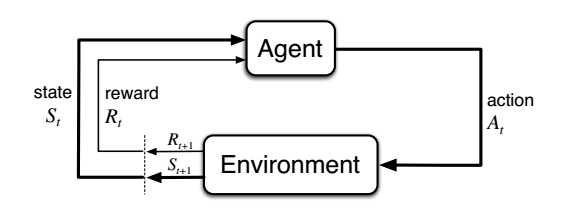
\includegraphics[width=350px,height=200px]{rl_diagram.png}
        \caption{RL}
        \label{fig:my_label}
    \end{figure}


"Reinforcement learning is learning what to do and how to map situations to actions so as to maximize a numerical reward signal" Sutton (pg 1)

A full discussion of reinforcement learning is not required to understand AlphaZero but it is necessary to look at the fundamental concepts that make up the algorithm. I present a sort hierarchy of concepts that are necessary to understand AlphaZero fully. It is possible to read through the paper or a tutorial to get the mechanics of the algorithm but to understand the "why" you will need to go deeper. 

    \begin{figure}[H]
        \centering
        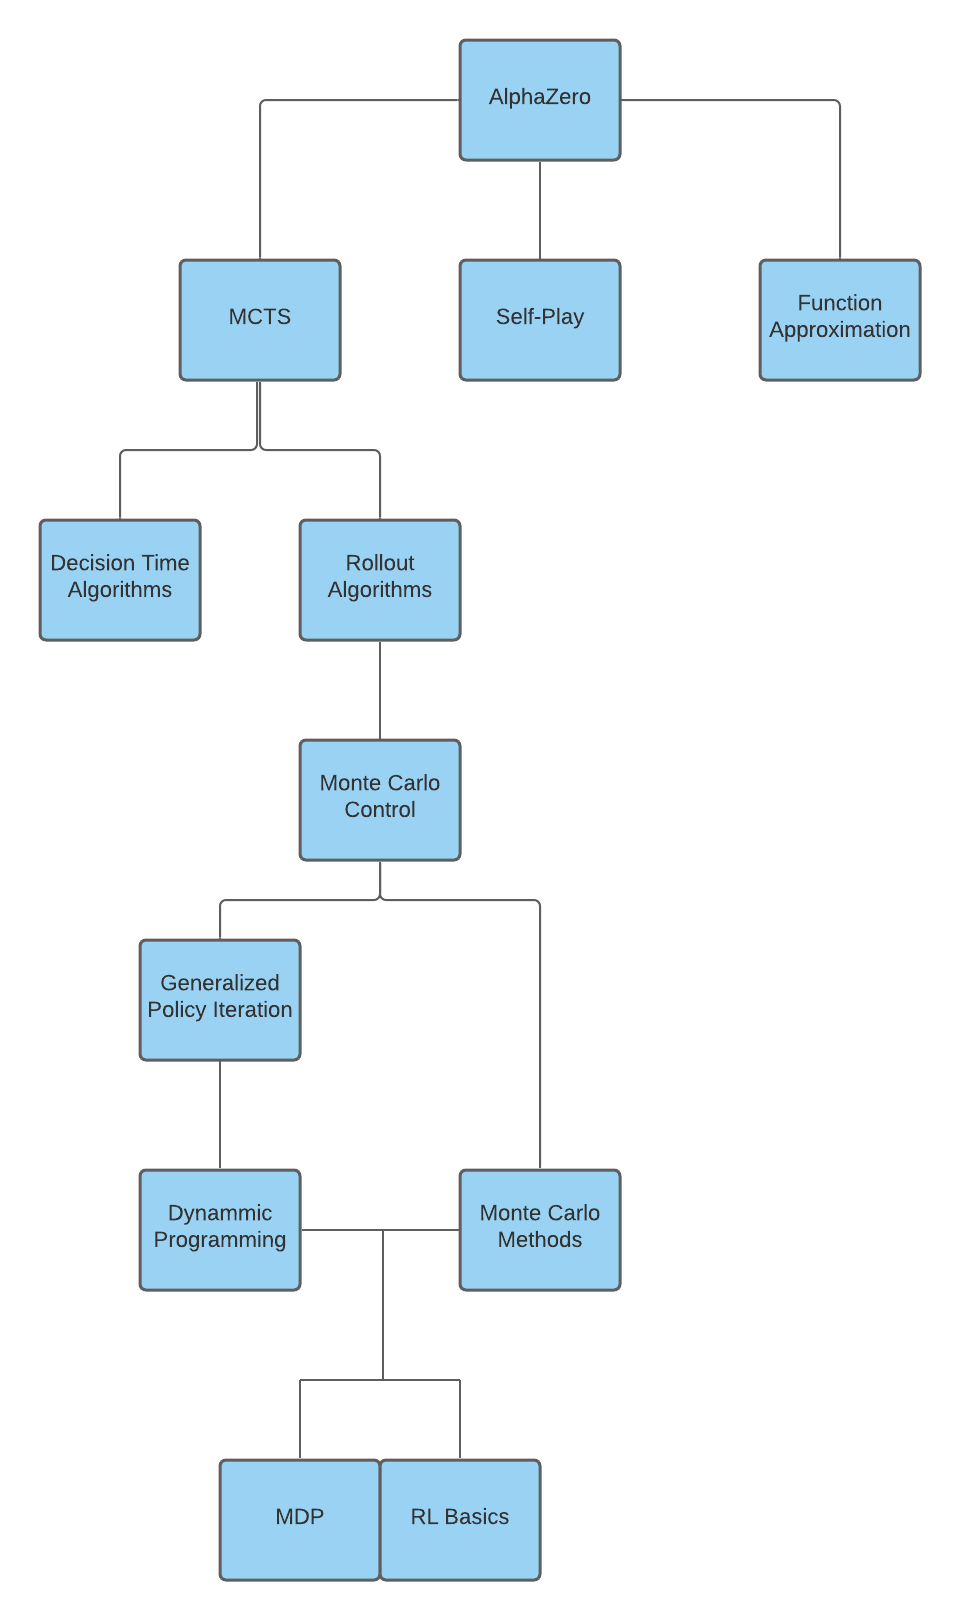
\includegraphics[width=350px,height=200px]{images/alphazero_concepts.png}
        \caption{Concept Hierarchy}
        \label{fig:my_label}
    \end{figure}

    
    \begin{enumerate}
        \item Environment
        \item State
        \item Policy
        \item Reward Signal 
        \item Value
        \item Model
    \end{enumerate}
    
    \subsection{Environment}
    
    Loosely defined as the thing that the agent interacts with. Everything that is exterior to the agent. The environment typically encompasses the system that is trying to be solved. It also provides observations and rewards as the agent takes actions. For example when trying to solve the game of Go the agent (the players) takes actions (moves pieces) and the environment is the board, the pieces, and the mechanism for telling the agent the current reward (win / loss) or other special states that are specific to the game. So it is the game itself plus a few other mechanisms to make the learning process possible. The environment is not synonymous with state as observed by the agent. We will look at that next. 
    
    \subsection{State}
    
    State is the representation of all information that is available to the agent at any given time. As said above this is not necessarily the same as the observation provided by the environment. For instance in AlphaGo Zero we will see that the state is actually a function of the current board as well as previous board positions. It is up to the designer of the reinforcement learning algorithm as to what is the best state to present to an agent. In many environments the choice might be more obvious than others. 
    The fact that state is something that needs to be decided upon by the designer of the algorithm hints at a potential need for more generalization within algorithms. MuZero and similar algorithms take a step in this direction by having the agent learn that representation. MuZero as will be discussed towards the end of this paper searches in a latent space. So the state as provided by the environment is projected onto a latent space and then the algorithm searches within this space. This is an interesting approach. For further discussion on this see \cite{predictron,muzero}
    
    \subsection{Policy}
    
    A policy roughly speaking is just a definition of an agents behavior given a perceived state of the environment. That is it is a mapping $ \pi: s \rightarrow a $ where s is a state of the environment and a is an action  $ a \epsilon A $. A is the possible set of actions the agent can take. It can be either discrete or continuous. In AlphaGo Zero actions are integers representing the place on the board.
    
    \subsection{Reward Signal}
    
    A reward signal is what defines the goal of a RL algorithm. As an agent observes an environment it receives feedback in the form of rewards. Generally an agent is simply trying to maximize the sum of its reward over the long run. Rewards help the agent to learn a policy. An agent will adjust the actions that it takes based off of the feedback it receives. Roughly speaking the agent will adjust to take actions more frequently that it perceives to return more reward. In environments like AlphGo Zero there is what is called the "sparse rewards" problem. This means that the agent might be interacting with the environment for long extended periods of time before receiving any feedback. 
    
    
    \subsection{Value}
    
    The value of a state in reinforcement learning is the amount of reward an agent should expect to receive in the long run from a given state. An agent is not given this number and is something that needs to be learned. This is generally expressed like this $ V(s) \rightarrow \mathbb{R} $. 
    
    From Sutton
    $ v_{\pi}(s) = E_{\pi}[G_{t}| S_{t} = s]$
    
    
    \subsection{Model}
    
    A model from the perspective of RL typically refers to a predictive model of the environment. It is a way for the agent to predict the behavior of the environment. This allows the agent to make inferences about what will happen when certain actions are taken. This in turn allows the agent to plan based on the model. Algorithms that use models are called \textit{model-based}. Algorithms that dont explicitly model the environment are called \textit{model-free}. The line between the two can easily become blurred as a lot of algorithms will mix between the two approaches. In the context of this paper AlphaZero and can be viewed as a Model free algorithm and MuZero as a model based extension to AlphaZero. MuZero attempts to learn the dynamics of the environment from scratch whereas for AlphaZero the dynamics are known upfront.  


\section{Markov Decision Processes}

The following section draws pretty heavily from Sutton \cite{sutton}. Lets put some of the previous concepts together into a framework that we can actually use to make decisions. Markov decision processes (MDP) are an idealized environment for making sequential decisions. MDPs have been studied quite thoroughly and although their formulation is simple it is also quite robust and a surprisingly large number of problems can be formulated as MDPs. Figure 2.1 that we looked at before is an example of a MDP. What kind of data would we get if we allowed the process in that figure to go on for many time steps? First the agent begins in the start state $S_{0}$ and takes action $A_{0}$ and receives a reward $R_{1}$ and the next state $S_{1}$. Then the agent would take another action $A_{1}$ and so on. This would result in a series of data points $S_{0},A_{0},R_{1},S_{1},A_{1},R_{2},S_{2},A_{2}....R_{T},S_{T}$. Here there is some terminating condition at time $T$ but the series could also just go on continuously. $R_{t},S_{t}$ are both random variables whose probability of occurrence only depends on the previous action and reward. This is what makes the process markovian and is called the Markov property. The only thing that matters in determining the probability of the next state and reward is the current state and action. The dynamics of this process can be described by a function $p: S x R x A x S \rightarrow [0,1] $. The function can be defined in terms of conditional probability. 

$$ p(s^{'},r | s, a) = Pr\{S_{t + 1} = s^{'}, R_{t + 1} = r | S_{t} = s, A_{t} = a\}$$

So the probability given by $p$ describes the entire environment dynamics. The Markov property as described in Sutton {Introduction to reinforcement learning} "is best viewed as a restriction not on the decision process, but on the state. The state must include information about all aspects of the past agent–environment interaction that make a difference for the future".

How state, action and time is defined is quite flexible in this formation. Time does not have to refer to an actual interval of time but can just be some set of steps that happen one after the other. Actions likewise can really be any decision that we want to learn how to make. 

Now that we have defined the system what is the actual goal? We want to get as much reward as possible. That means no just the reward that we receive right now but all the reward we accumulate. This statement results in the \textit{reward hypothesis} {Introduction to reinforcement learning}

\say{..what we mean by goals and purposes can be well thought of as the maximization of the expected value of the cumulative sum of a received scalar signal (called reward)}.

Since learning from rewards has become so popular it might not seem like that strange of a concept and indeed it might be fairly intuitive. However this is one of the things that distinguishes reinforcement learning from other forms of machine learning. In a typical supervised learning setting for instance you attempt to minimize a loss function on a set of observed data w.r.t to some given labels. Like attempting to predict credit card fraud from a set of features. You are first given a bunch of examples with labels as to whether fraud occurred in that particular instance. You then want to train a model to be able to generalize from these observed features and labels to unlabeled or data that has not been seen yet. Reinforcement learning is different in that we dont generally start out with a set of features and labels. The agent produces data or observation as we act in the environment. Then through these observations we change the agents behavior as to achieve a desired goal. There is a bit of an art in setting up the rewards correctly. The designer of the algorithm has to choose the rewards for an environment and it is not always trivial. For GO and other two player zero sum games it is natural to assign a reward of +1 for winning, -1 for losing and 0 for a draw. You might however want to assign a small amount of reward to a draw so that the agent is receiving some amount of feedback. You might want to set up intermediate goals as to "show" the agent the right choices to make or steer them away from obviously bad choices. An example of a miss application of reward assignment would be in chess to give reward to an agent for pieces captured. This can lead the agent to commit detrimental errors to the main goal of winning just to achieve the sub goal so care must be taken that the subgoals align with the main goal. 

In this paper we will be focused on situations in which there is a clear start and end state. There are of course other domains in which this is not the case. Self-driving cars, trading in markets, and playing atari games are a few examples. Since we are trying to maximize an accumulated reward we can define our main goal as the following. 

\begin{equation}\label{Cumulative sum}
 G_{t} = \sum_{k=t + 1}^{k=T} R_{k}
\end{equation}

There is something still not quite right here. In this formulation we would value rewards at all time steps equally. This is usually not the case in most tasks however. The idea that 100\$ today is better than 100\$ 10 years from now applies here. Typically the reward we get now is more valuable then the same amount in the future. So we can modify our goal a bit by discounting rewards that we receive farther into the future. We do this by using a discount factor $\gamma < 1$. 

\begin{equation}\label{Discounted Cumulative Sum}
G_{t} = \sum_{k=t + 1}^{k=T} \gamma^{k - t + 1} R_{k}
\end{equation}

Ok, great we have a goal now how do we use that goal to start defining how the agent is going to behave? Well we want the agent to take actions that are going to lead to higher $G$. Taking actions in our MDP formulation leads us to end up in different future states. So we want to end up in better states. What does it mean to be a better state? A better state is one that leads to more $G$. So we want to be in states in which we expect to collect more reward in the future. Lets try and put this into something concrete. The expected value of a state seems to fit well into what we are going after so we can use that as a starting point. 

\begin{equation}\label{Expected State Value}
\mathbf{v}_{\pi}(s) \dot{=} \mathbb{E}_{\pi}[G_{t} | S_{t} = s]
\end{equation}

The $\pi$ here refers to the policy of the agent. So this is looking at the expected value assuming the agent is following a given policy. We discussed policies previously and we will discuss them more in the future. It is important for knowing the expected value while following an MDP because a policy will define how we transition from one state to the next. We can also define a value function for a state action pair in a similar manner. 

\begin{equation}\label{Expected State Action Value}
\mathbf{q}_{\pi}(s,a) \dot{=} \mathbb{E}_{\pi}[G_{t} | S_{t} = s, A_{t} = a] 
\end{equation}

Its quite easy to see that if one actually had access to one of these functions how you might have the agent behave. In the case of $\mathbf{q}_{\pi}$ simply pick the action with the largest value. We of course don't have access to these and have to learn them from experience. How might we do this? One way is to somehow track the average return that you get from a particular state or state action pair. This approach is called Monte Carlo methods. This is quite relevant for understanding AlphaZero as a form of tree search called Monte Carlo tree search is central to the algorithm. 
    
One central idea in reinforcement learning is the ability to view a value function recursively. Lets look at how we can do that. First we can write our cumulative variable $G_{t}$ in terms of the next immediate reward and a discounted cumulative return starting from the next timestep.  

    $$ \mathbb{E}_{\pi}[G_{t} | S_{t} = s] = \mathbb{E}_{\pi}[R_{t + 1} + \gamma G_{t + 1} | S_{t} = s] $$
    
Then we can expand this by thinking about what en expectation means here in terms of our random variable $R_{t + 1}$. In words it is the value of all future rewards we would see by transitioning to new states. We have said previously that the probability of transitioning to a new state $s^{'}$ and receiving reward $r$ from the current state given a certain action is given by the function $p(s^{'},r|,s,a)$ the system dynamics of our MDP. We know the definition of expected value is the sum over possible outcomes of a random weighted by the probability of that outcome happening. So we can write the expected value of $R_{t}$ given a specific state and action. 

$$ \mathbb{E}[R_{t}] = \underset{s^{'},r}{\sum}p(s^{'},r|,s,a)[ r ]$$

We want however to look at the expectation following a specific policy. A policy $\pi(a|s)$ gives us a distribution over possible next actions given the current state. So we can further expand on our previous equation. 

$$ \mathbb{E_{\pi}}[R_{t}] = \underset{a}{\sum}\pi(a|s)\underset{s^{'},r}{\sum}p(s^{'},r|,s,a)[ r ]$$

We can now go back to our expectation of the cumulative reward. 

$$\mathbb{E}_{\pi}[R_{t + 1} + \gamma G_{t + 1} | S_{t} = s] = \underset{a}{\sum}\pi(a|s)\underset{s^{'},r}{\sum}p(s^{'},r|,s,a)[ r + \gamma \mathbb{E}_{\pi}[G_{t + 1} | S_{t + 1} = s^{'}]] $$

Notice how the expectation is now conditioned on the next state. This allows us to rewrite this in a recursive form.

\begin{equation}\label{Bellman State Value Equation}
\mathbf{v_{\pi}(s)} = \underset{a}{\sum}\pi(a|s)\underset{s^{'},r}{\sum}p(s^{'},r|,s,a)[ r + \gamma \mathbf{v_{\pi}(s^{'})}]
\end{equation}

This last form is know as the bellman equation. The bellman equation represents values of a state in terms of values of future states. The figure below taken from Sutton represents this as a decision tree. The open circles are states and the black circles are actions. This shows if you are in state $s$ you have 3 actions that are part of policy $\pi$. Once you take one of those actions the environment then transitions to one of two next states $s^{'}$ and emits a reward $r$ with probability $p$. You could then extend the diagram in the same way from each of the next states. If this were a two player game the other player would be part of the environment and the probability of transition to state $s^{'}$ would depend on the other players policy $\pi$. Sutton refers to these as backup diagrams because they show how information could be propagated back up the tree. 

\begin{figure}[H]
        \centering
        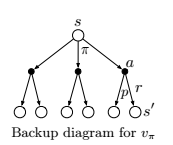
\includegraphics[width=350px,height=200px]{images/bellman_update.png}
        \caption{RL}
        \label{fig:my_label}
\end{figure}

\section{Tictactoe Bellman Equation}

Lets try and picture what the bellman equation might look like for the game of tictactoe. This example will help to both illustrate how the equation works and also the intractability of calculating it in practice. The figure below shows the initial blank board at the beginning of the game. To calculate the value of this position we will do so from player X's perspective. There are nine possible next moves and so each of those needs to be assigned a probability represented by the policy $\pi(a | s_{0})$. Then focusing on action $a_{0}$ at the top of the diagram the next thing we would need to do would be to calculate $p(s^{'},r|,s,a)[ r + \gamma \mathbf{v_{\pi}(s^{'})}]$ for each of the possible next states. So we could start with $p(s_{1},r|,s_{0},a_{0})$. What is this probability? We will need to know this beforehand. How it is obtained depends. We might just be given the distribution beforehand as part of our model of the environment. In this instance however a more intuitive candidate would be to ask player "O" for their policy. That is if we had access to $\pi$ from player "O" perspective that would be then give the associated probability of future states since future states are just the board after "O" has chosen an action. Now that we have $p(s_{1},r|,s_{0},a_{0})$ we need $[r + \gamma v(s_{1})]$. The reward $r$ here refers to the immediate reward observed. In the case of tictactoe and most other two player board games there will be no reward till the end of the game. So $r$ here is just 0. So we need $\gamma v(s_{1})$. Here $\gamma$ is a discount factor and is constant and chosen beforehand. The $v(s_{1})$ calculation is shown next. 

\begin{figure}[H]
        \centering
        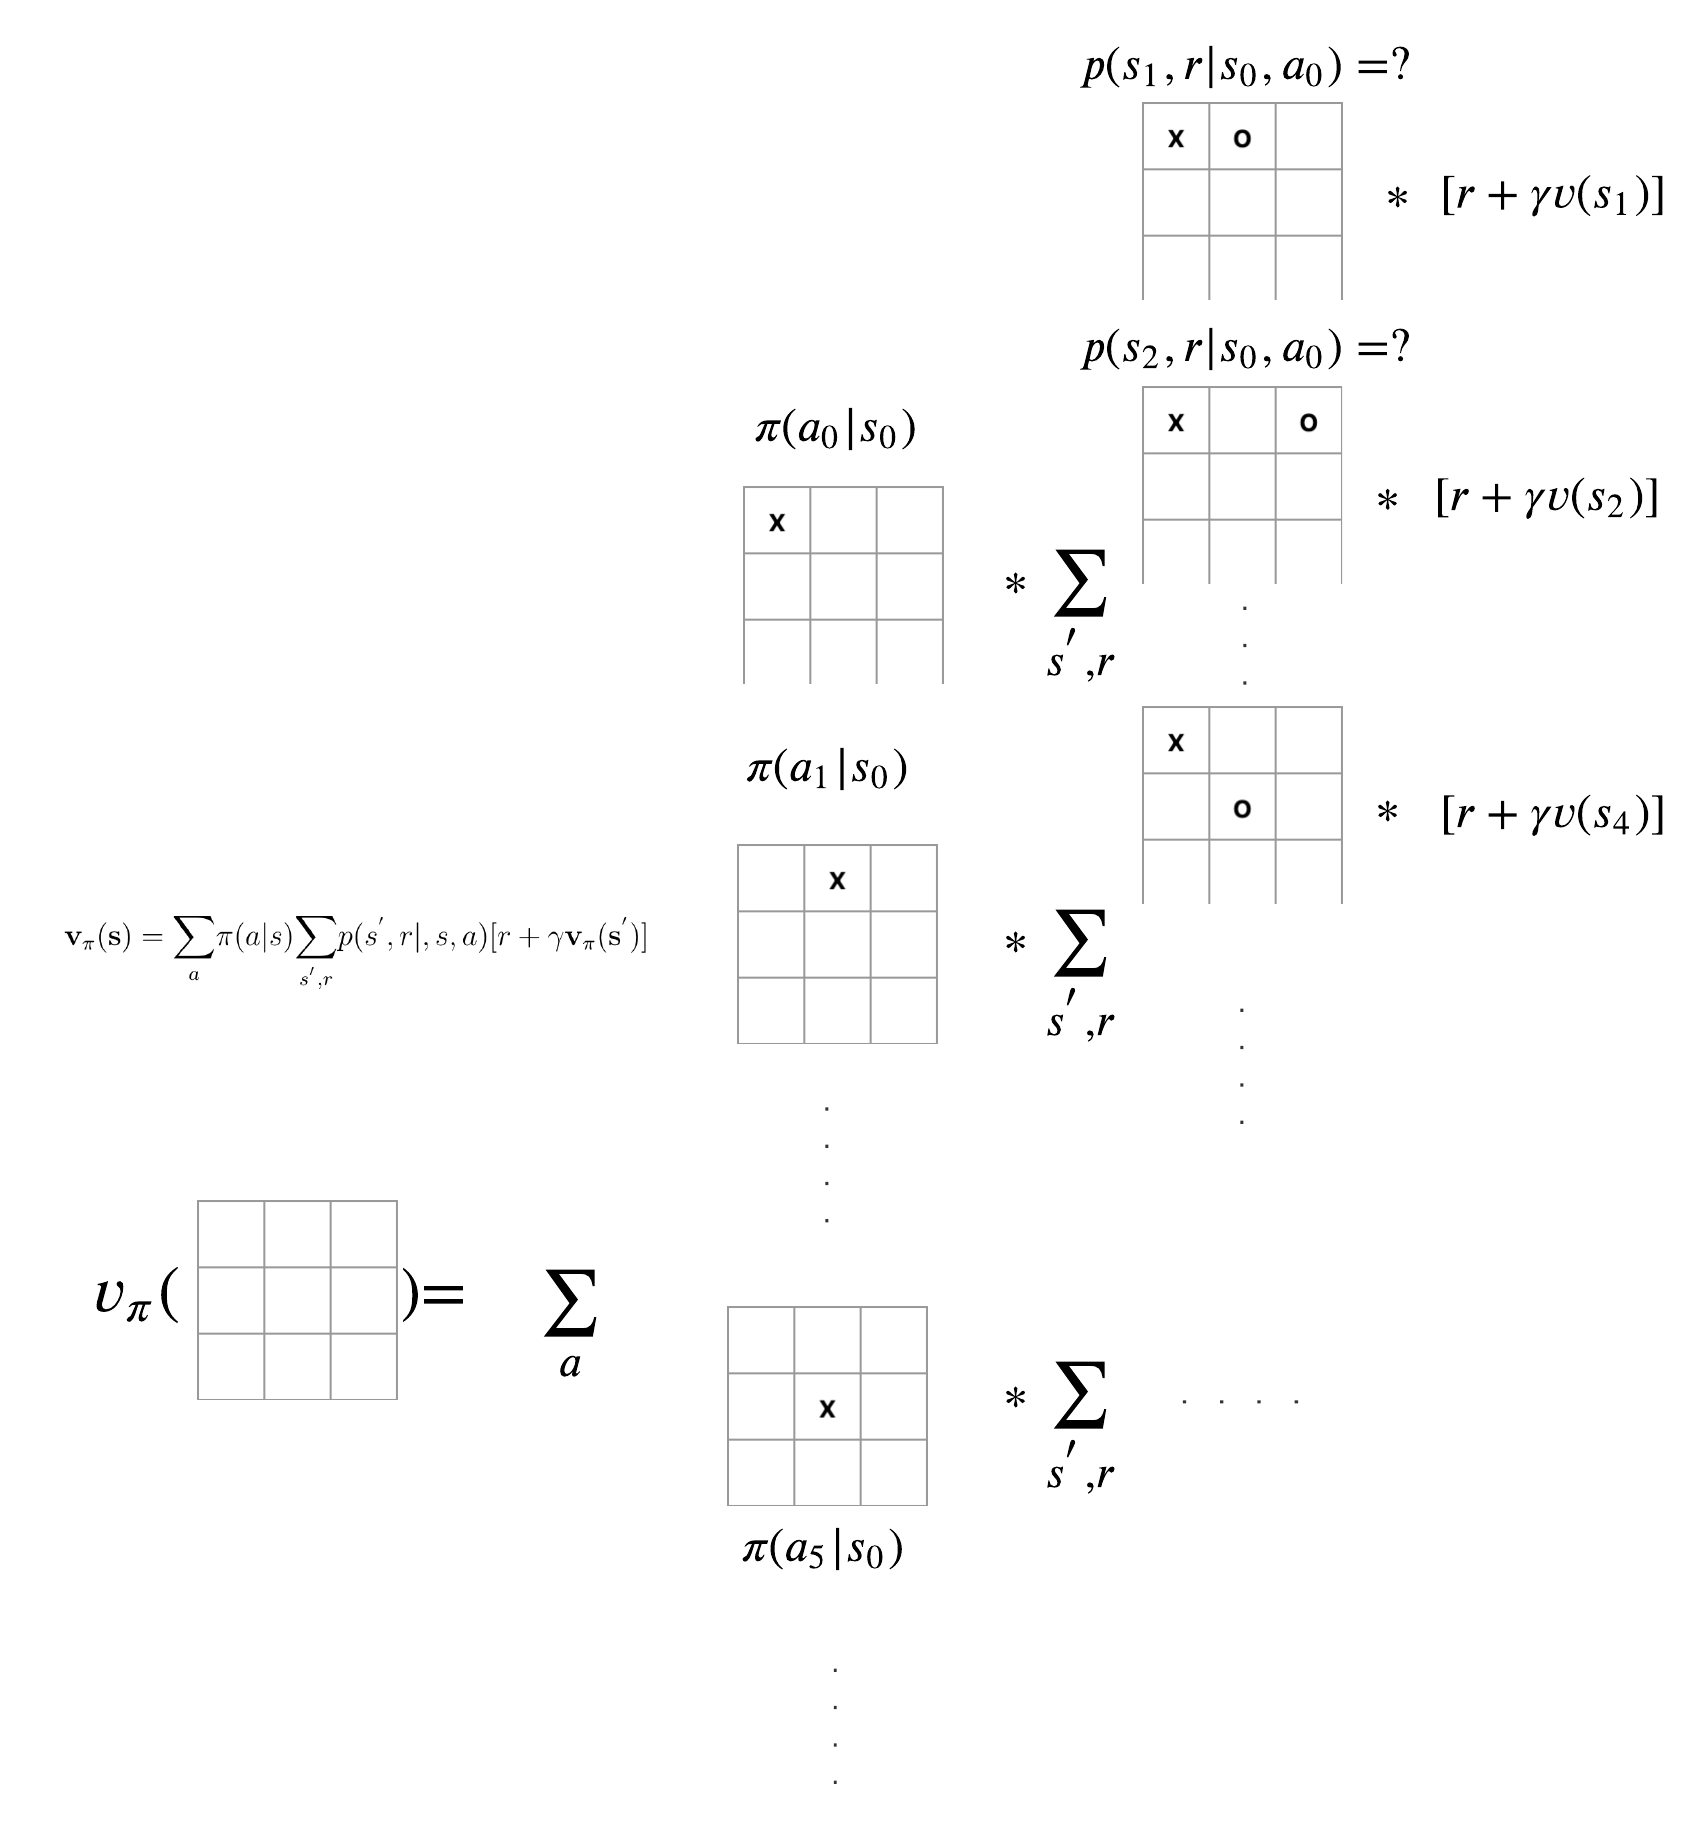
\includegraphics[width=400px,height=300px]{images/PolicyEvaluationExample/intractable_value_function.png}
        \caption{}
        \label{fig:my_label}
\end{figure}

In figure 2.5 below we see the same calculation expanded out but for state $s_{1}$. This same sort of recursive procedure would keep going until a terminal state was reached. For tictactoe this occurs only when the game ends and a reward of 1,-1 or 0 is assigned for win,loss or draw. 

\begin{figure}[H]
        \centering
        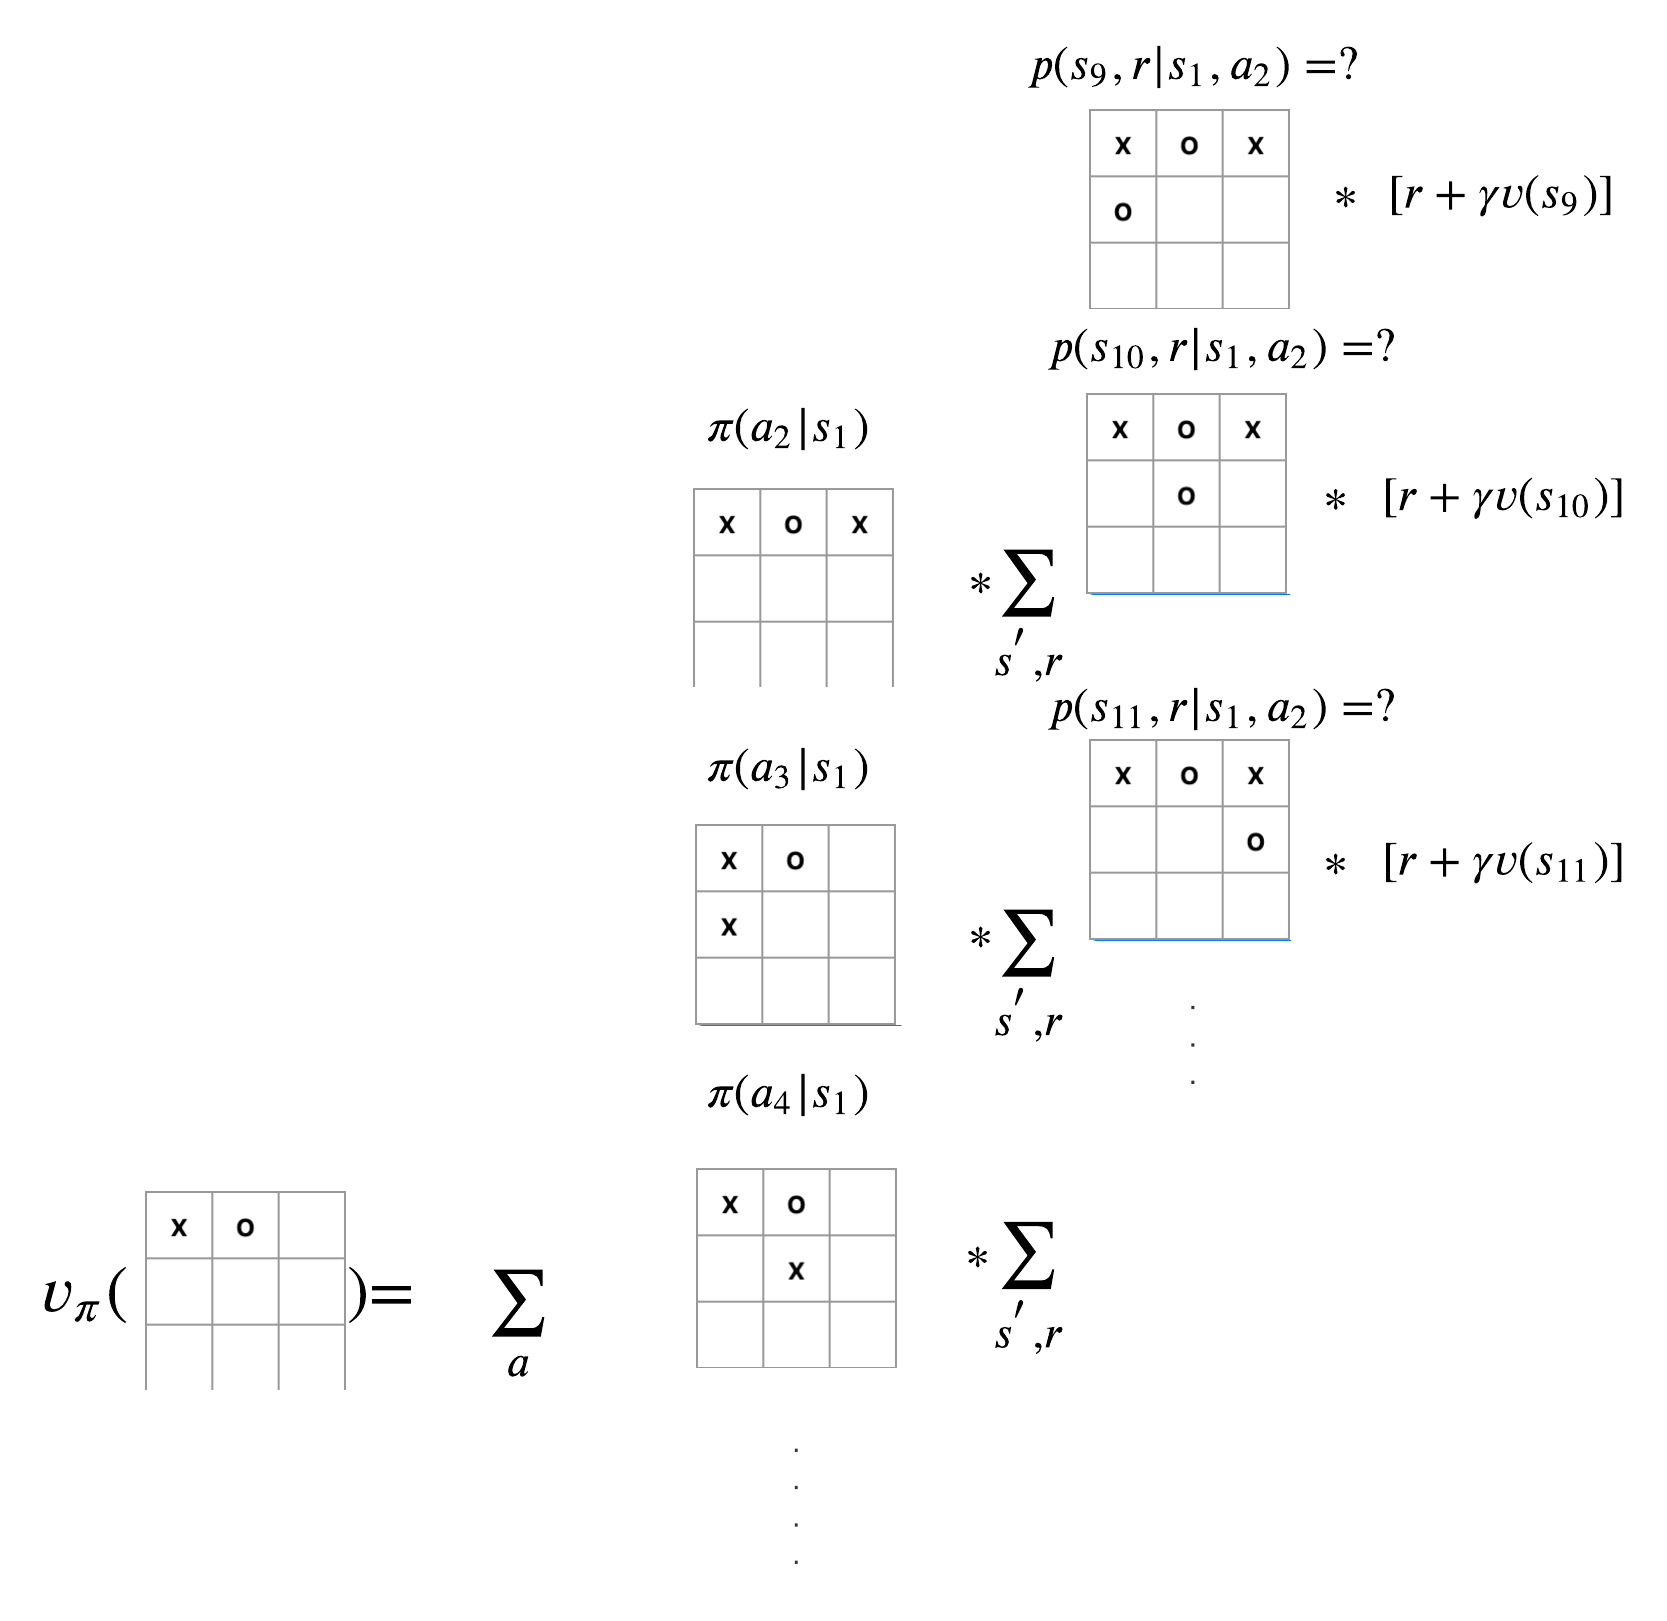
\includegraphics[width=400px,height=300px]{images/PolicyEvaluationExample/intractable_value_function_2.png}
        \caption{}
        \label{fig:my_label}
\end{figure}

\section{Policy evaluation Example}

Lets look at an example of evaluating this a value function for a specific state and policy using a more simple tictactoe example as a test case. Consider the board below. It is player X to go. How to you calculate equation (2.5)? Once again we need access to a policy and access to the transition probability distribution. 

\begin{figure}[H]
        \centering
        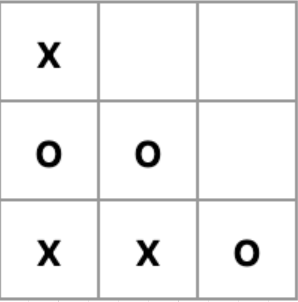
\includegraphics[width=150px,height=150px]{images/PolicyEvaluationExample/pe_example_s0.png}
        \caption{}
        \label{fig:my_label}
\end{figure}

Lets ignore that this is a two player game for a moment. From player X's perspective all we need is to set our own policy. Then the next state we observe after taking an action will be given by the environment. In this case player "O" will just be part of the environment. The situation is displayed in the figure below. We have three possible actions to take. We can see what the correct thing to do is but a computer has no idea! So lets assign probability $\frac{1}{4}$ to the top two actions and $\frac{1}{2}$ to the other action. When the agent takes action $a_{2}$ or the top right square he observes a next state $s_{1}$ and reward $-1$. This event happens with probability one and so no other events occur after taking that action. The same is shown for action $a_{1}$. For action $a_{5}$ the next state is observed but it is not a terminal state so a policy needs to be defined. There is only one action so the definition is simple. No next state is observed just a reward of 0 since it is a terminal state. Lets now actually calculate $v_{\pi}(s_{0})$ 

\begin{figure}[H]
        \centering
        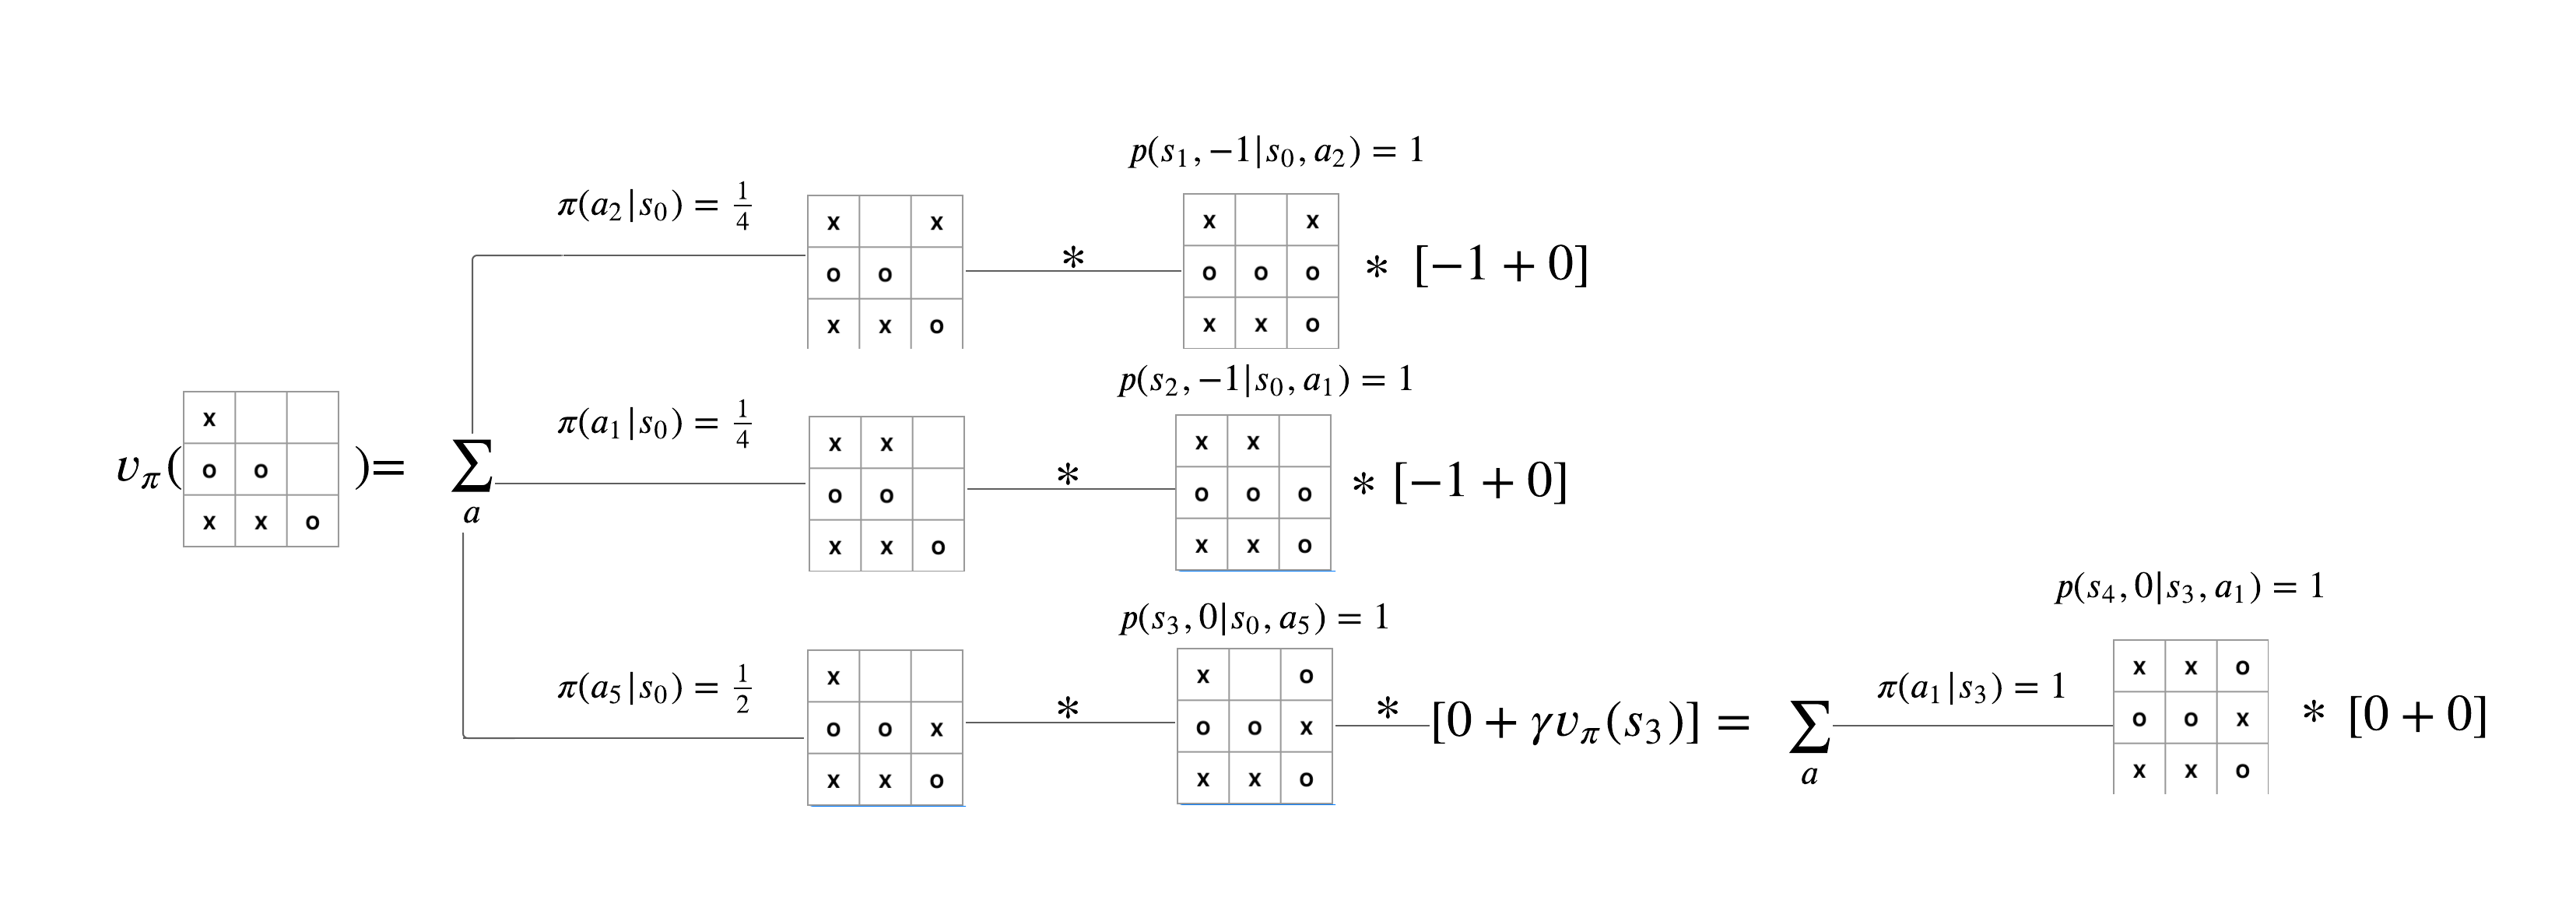
\includegraphics[width=400px,height=150px]{images/PolicyEvaluationExample/value_function.png}
        \caption{}
        \label{fig:my_label}
\end{figure}

Lets calculate the value of using this policy from the initial state using equation (2.5). With the small number of states being used this is a fairly easy calculation but its easy to see how this could easily start to become intractable. 

\begin{figure}[H]
        \centering
        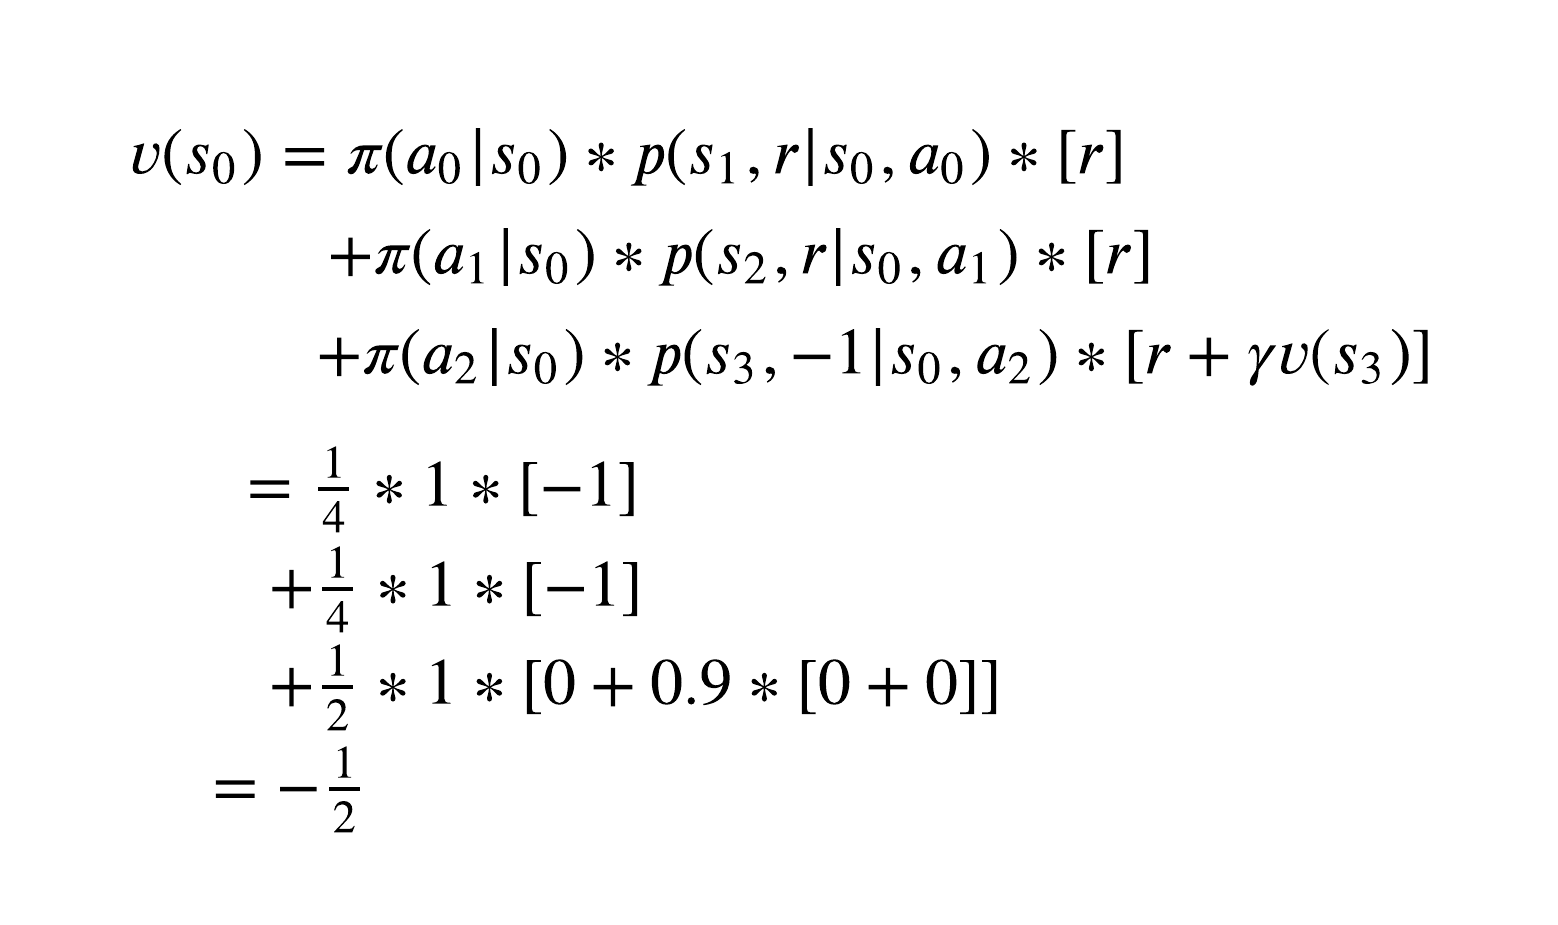
\includegraphics[width=400px,height=200px]{images/PolicyEvaluationExample/value_function_calc.png}
        \caption{}
        \label{fig:my_label}
\end{figure}

We have now discussed how to evaluate given states within our framework. We have not discussed yet how to actually use this information to make good decisions. There is a theorem in RL that says that a policy $\pi$ is better than or equal to another policy $\pi^{'}$ if its expected value is greater than or equal to the expected value of $\pi^{'}$ for all states. In other words $ \pi \geq \pi^{'} $ iff $ \mathbf{v_{\pi}}(s) >= \mathbf{v_{\pi^{'}}}(s)$ for all $ s \in  S$. It has also been shown and we will restate here without proof that an optimal policy always exists for an MDP. There can be more than one but at least one exists. The notation used for the optimal policy is usually $\pi_{*}$ and we will take that notation here as well. This leads also to the fact that there is an optimal state value function. 

\begin{equation}\label{Optimal State Value Equation}
\mathbf{v_{*}}(s) \dot{=} \underset{\pi}{max} \: \mathbf{v_{\pi}}(s) , \: \forall s \in S 
\end{equation}

The bellman equation representation must hold as well. In our previous representation of the bellman equation we had to sum over all actions from our policy $\pi(a |s)$. When looking at an optimal policy in the case of an MDP we will only be interested in taking the best action. So we can rewrite the bellman equation of the value function with that in mind. 

\begin{equation}\label{Optimal Bellman State Value Equation}
\mathbf{v_{*}}(s)= \underset{a}{max}\underset{s^{'},r}{\sum}p(s^{'},r|,s,a)[ r + \gamma \mathbf{v_{*}(s^{'})}]
\end{equation}


A similar analysis can be done for $q(s,a)$. We will not go through that here but you can look to Sutton or other sources for more discussion. We will simply present the result here. 

\begin{equation}\label{Optimal Bellman State Action Value Equation}
\mathbf{q_{*}}(s,a)= \underset{s^{'},r}{\sum}p(s^{'},r|,s,a)[ r + \underset{a}{max} \: \mathbf{q_{*}}(s^{'},a^{'})]
\end{equation}

I think that the $\mathbf{q_{*}}$ optimal value function can be more intuitive. It simply says that the value of the optimal action from the current state is a weighted sum over possible next states assuming we take the optimal action from those states as well. If you have $\mathbf{q_{*}}$ or $\mathbf{v_{*}}$ than coming up with the correct policy is easy. For $\mathbf{v_{*}}$ you just have to do one step look ahead to see which actions will give you the max. You dont have to continue to look further because you already have access to the optimal values of the next state. With $\mathbf{q_{*}}$ you simply look up the best action from the current state. No further search is necessary. Obtaining these optimal functions of course generally takes a lot of work and in any large setting is intractable to compute directly. To actually compute an optimal bellman equation you need to have perfect knowledge of the environment, sufficient resources and the markov property. These assumptions typically dont hold for most interesting problems. For any problem that breaks one of these assumptions some sort of approximation will be needed. One approach that fits in closely with the bellman optimality equation is dynammic programming which we will discuss shortly. One big takeaway from reading Sutton and others work is that most reinforcement learning techniques come down to different ways of approximating the bellman optimality equation. To me this is quite powerful and means that even though we might come across some powerful approximation techniques such as those that we see in AlphaZero they can all be viewed from the perspective of approximating the bellman equation in some way. 

\section{Dynamic Programming}

Dynamic programming (DP) is one of the more foundational topics within machine learning. We will not dwell on this topic too long but there are a few important lessons in which DP can help inform our understanding of RL and AlphaZero. We have just concluded discussing optimal value functions and now we need to find a way to actually compute them. That is where DP comes in. DP is essentially a collection of algorithms used to compute optimal value functions. Recall that (\ref{Bellman State Value Equation}) gave us a way to evaluate the value of state given a certain policy. This equation actually gives us a system of linear equations and can be solved directly if the model of the environment is totally known. We have $|S|$ equations and $|S|$ unknowns. This of course is not computationally very feasible so we need to find a way to compute (\ref{Bellman State Value Equation}) iteratively. We can actually just turn it into an update rule like the following. 

\begin{equation}\label{Bellman State Value Update Equation}
\mathbf{v_{k + 1}(s)} = \underset{a}{\sum}\pi(a|s)\underset{s^{'},r}{\sum}p(s^{'},r|,s,a)[ r + \gamma \mathbf{v_{k}(s^{'})}]
\end{equation}

We can first initialize $v_{0}(s)$ for each state randomly. We can use domain knowledge to set reasonable initial values as well or just set everything to 0 to start. This iterative process will converge to $v_{\pi}$ as $ k \rightarrow \infty$. This is called \textit{iterative policy evaluation} and it gives us a way to evaluate the current policy $\pi$ in an iterative fashion. We of course dont have to wait for $ k \rightarrow \infty$. In practice we can implement some stopping condition for which we are satisfied that $v_{k}$ is close enough to $v_{\pi}$. 

We dont want to just know the value of a given policy however we want to find what the best policy is. So we need to find a way to update our policy as well. I will state here what is known as the \textit{policy improvement theorem}. 

\newtheorem{remark}{Policy Improvement Theorem}

\begin{remark}\label{Policy Improvement Theorem}
Let $\pi$ and $\pi^{'}$ be any two separate deterministic policies for all $s \in S$ s.t. $q_{\pi}(s,\pi^{'}(a)) \geq v_{\pi}(s)$. Then the policy $\pi^{'}$ is greater than or equal to $\pi$. This implies that $ \forall s \in S$ each state value function has the relationship that $v_{\pi^{'}}(s) \geq v_{\pi}(s)$
\end{remark}

The idea here is that if you can take a policy $\pi$ and change one of its actions at a particular state to guarantee that it is at least as good or better than $\pi$ at that state then you can just change the policy at that particular state to the new action and you now have a better policy $\pi^{'}$. How can we do this at every state to give us a general methodology? We can do whats called acting greedily. Acting greedily means that from a given state you take the action that maximizes return from a one step look ahead perspective according to $v_{\pi}$. We can adjust (\ref{Bellman State Value Equation}) once again to represent this. 

\begin{equation}\label{Greedy Policy}
\mathbf{\pi^{'}} = \underset{a}{argmax}\underset{a}{\sum}\pi(a|s)\underset{s^{'},r}{\sum}p(s^{'},r|,s,a)[ r + \gamma \mathbf{v_{\pi}(s^{'})}] = \underset{a}{argmax} \: \mathbf{q_{\pi}(s,a)}
\end{equation}

This just says what we have already said in words. We use the current policy $\pi$ and take the action that is going to maximize our policy evaluation from a given state using $\pi$. This gives us a new policy $\pi^{'}$ that we know from the policy improvement theorem will guarantee us an improved policy. The only way its not an improvement once again is if we already had an optimal policy. Now that we have a new policy $\pi^{'}$ how can we continue to improve it. We need to evaluate $\mathbf{v_{\pi'}}$ using policy evaluation. Then we can use (\ref{Greedy Policy}) again to get a new policy $\pi^{''}$

$$ \mathbf{\pi^{''}} = \underset{a}{argmax}\underset{a}{\sum}\pi^{'}(a|s)\underset{s^{'},r}{\sum}p(s^{'},r|,s,a)[ r + \gamma \mathbf{v_{\pi^{'}}(s^{'})}]
$$

We can then repeat this process until convergence. This algorithm is called \textit{}{policy iteration} and is given in full below. 

 \begin{figure}[H]
        \centering
        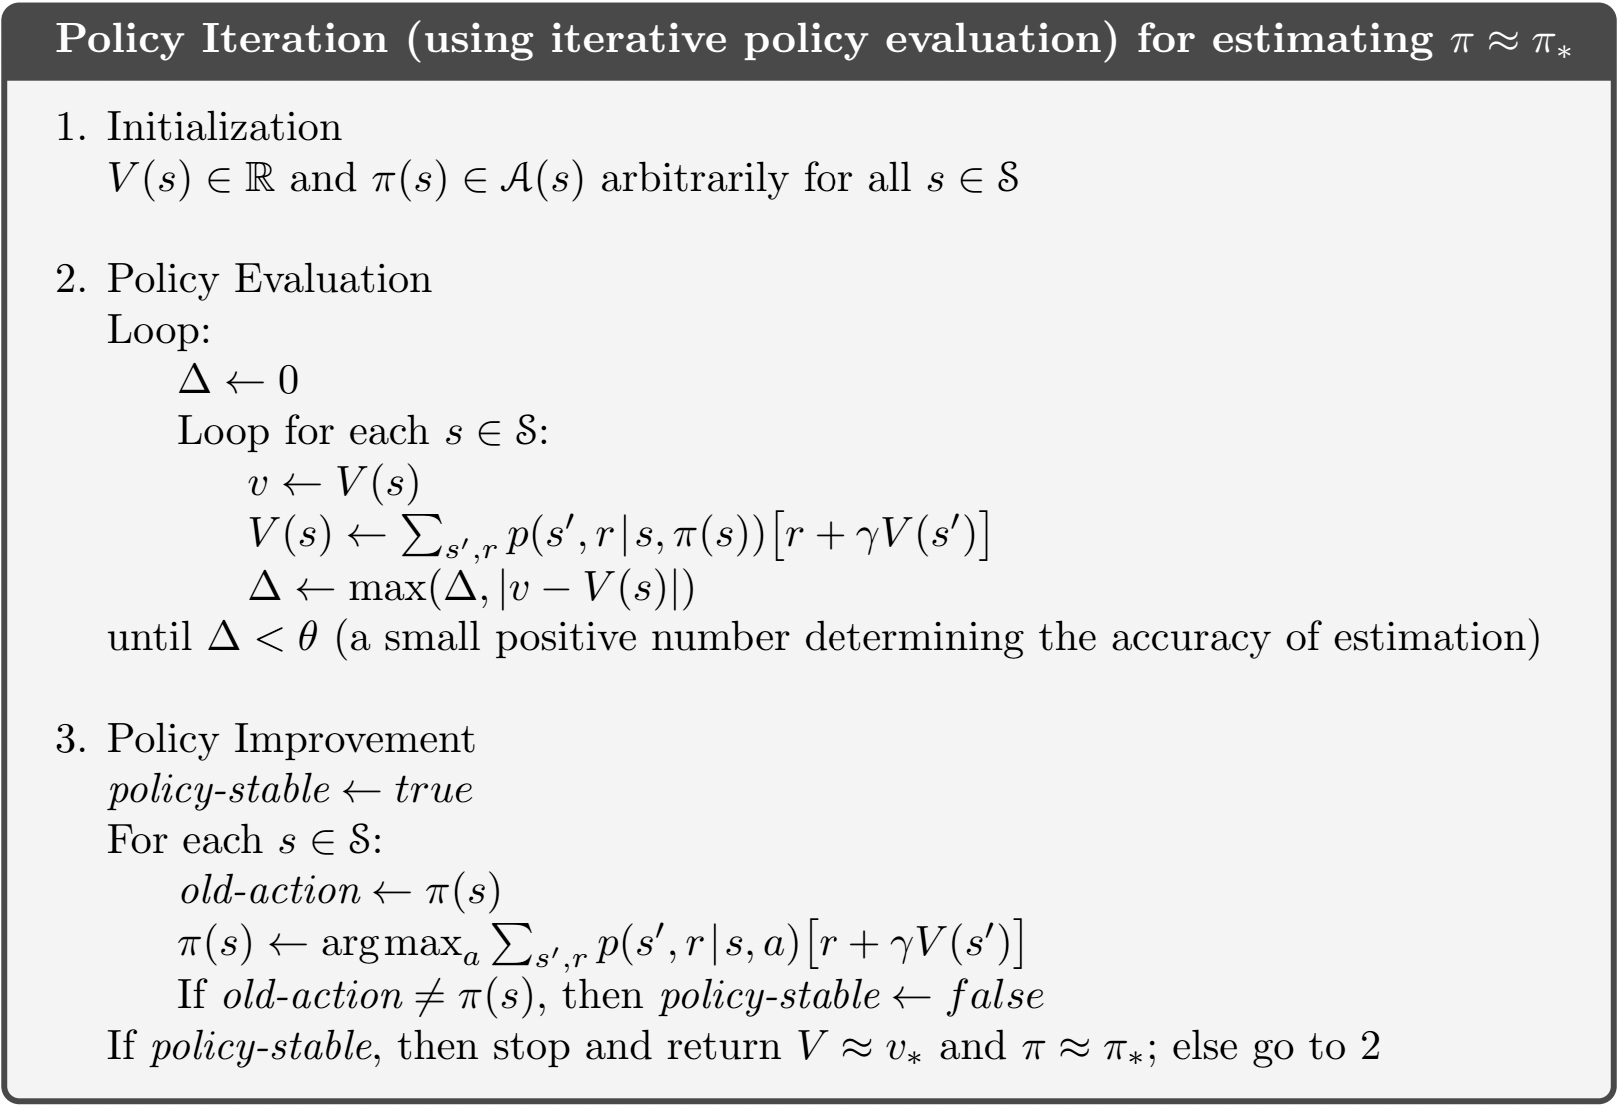
\includegraphics[width=350px,height=200px]{images/policy_iteration.png}
        \caption{From Sutton Chpt 4.3}
        \label{fig:my_label}
    \end{figure}

This idea of iterating back and forth between evaluation of a policy and improving a policy is a fairly general concept. In fact there is something called \textit{General policy iteration} (GPI) which captures these two concepts. Many reinforcement learning algorithms can be described in terms of GPI. The process is quite interesting because as soon as you perform policy improvement your value function is no longer accurate because it is still in reference to the old policy. So then you update the value function with the new policy to make it accurate again. The policy however is no longer optimal w.r.t the current value function so you adjust the policy by once again acting greedily. This goes back and forth until convergence is reached. There is a constant pushing and pulling between policy evaluation and policy improvement. 



\section{Monte Carlo Methods}

Monte Carlo in regards to reinforcement learning is a bit more specific than its typical meaning. In this discussion by "Monte Carlo" we mean any method that uses an average return for estimation. We will focus on estimating the value $\mathbf{v}_{\pi}(s)$ of a particular state. We said that our goal with $\mathbf{v}_{\pi}$ was to compute the expected value of the cumulative returns from a particular state. To apply monte carlo methods to this problem we can just track the average return we observe when visiting that particular state. We can do this directly from experience assuming the agent is following the policy $\pi$ and in the limit we should have a true estimate of $v_{\pi}$. This is called Monte carlo prediction and the most common form is called first-visit. This means that we simply average the return from the first visit to a particular state. For every visit we average the return following every visit. The first-visit method  has better understood theoretic properties. Every-visit however extends more naturally to function approximation. They both however converge to $\mathbf{v}_{\pi}(s)$ as the number of visits goes to infinity. The outline of the algorithm taken from Sutton is displayed below. 

\begin{figure}[H]
        \centering
        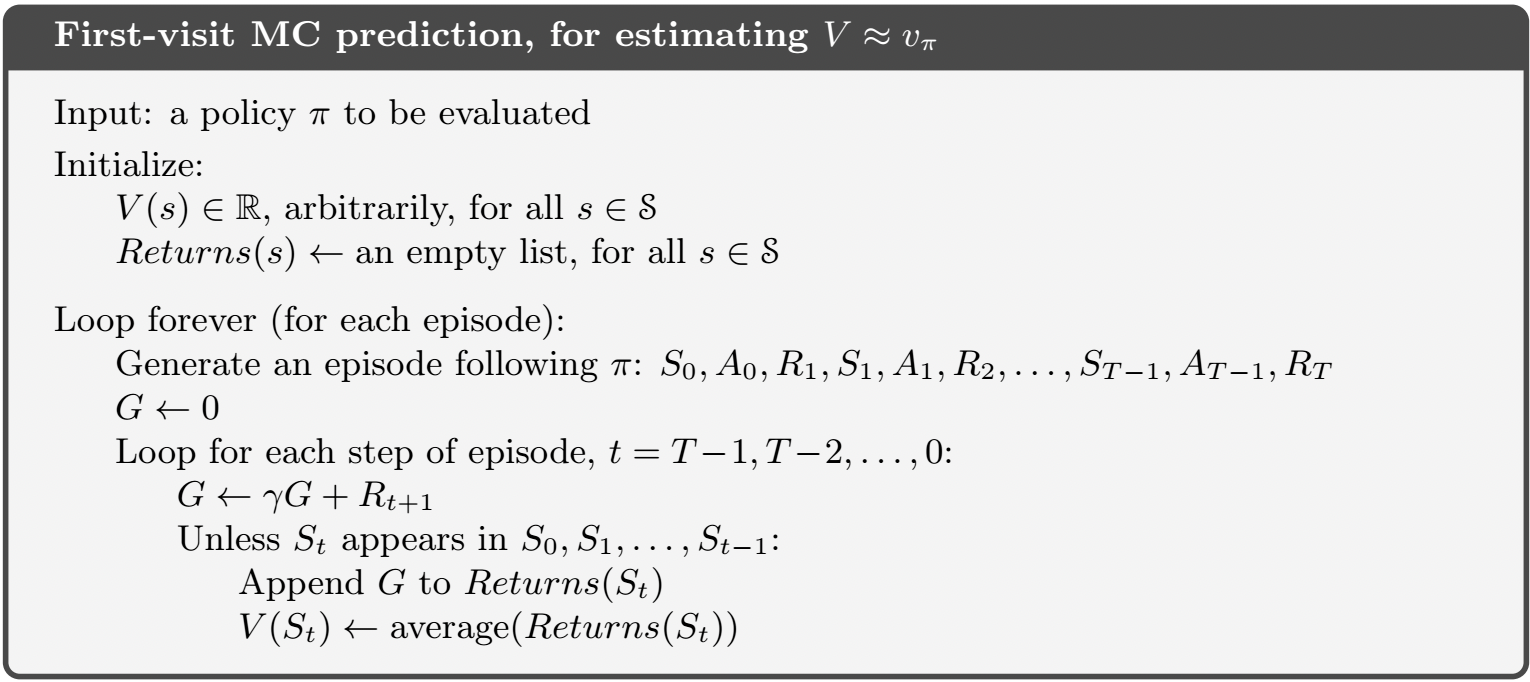
\includegraphics[width=350px,height=200px]{images/first-visit-mc.png}
        \caption{First-visit MC prediction}
        \label{fig:my_label}
    \end{figure}

Some important facts about MC methods

\begin{enumerate}
    \item One advantage of MC prediction is that we dont need to have a complete model of the environment in order to come up with an estimate for the state $s$. Since Monte Carlo Methods work with sample episodes they simply can use a given policy to keep generating samples.
    \item MC methods always run to the end of an episode whereas DP only looks one step ahead. 
    \item The estimate for each state is independent. For DP this is not the case because DP bootstraps
    \item Computational expense of estimating the value of a state is independent of the number of states
\end{enumerate}

Advantages over DP

\begin{itemize}
    \item Can learn from actual experience
    \item Can learn from simulated experience
    \item Can generate sample episodes starting from some state that your interested in and just average return from only that state and ignore the rest. 
\end{itemize}
 
Just like we saw with DP we can move from simply evaluating a given policy to actually attempting to find a best policy. We say that General policy iteration (GPI) was a flexible way of framing the problem. We can do a similar thing with MC methods. Just as before we can improve the policy by simply acting greedily w.r.t the value function $q(s,a)$. It is easier to frame a GPI model for MC methods in terms of the action-value function $q_{\pi}$ instead of $v_{\pi}$ which requires us to do a lookahead search.  So the greedy policy is defined as 


\begin{equation}\label{MC Greedy}
\pi(s) \dot{=}\underset{a}{argmax} \: q(s,a)
\end{equation}

The policy improvement theorem as discussed before applies to $\pi_{k}$ the $kth$ step of the algorithm. This means that if at each iteration of the algorithm we improve our policy by acting greedily than we can assume that the following is true. 

$$
q_{\pi_{k}}(s,\pi_{k + 1}) \geq \mathbf{v}_{\pi_{k}}(s)
$$

There are two assumptions here that are necessary for convergence. The first is that sufficient exploration is happening. That is that each state action pair has some non zero probability of occurring. The second is that we need an in order to evaluate a given policy we need an infinite number of episodes. The Monte Carlo Exploring Starts algorithm is an example of one that drops the second requirement but satisfies the first by randomly choosing a state action pair to start at. The value function $Q(S_{t},A_{t})$ is able to converge accumulating and averaging returns for all episodes. Convergence although intuitively seems guaranteed has not so far been proven. The exploring starts assumption can be dropped by doing things like using a $\epsilon$-greedy algorithm that with probability $\epsilon$ takes a random action. This will ensure that all state action pairs are visited in the limit and allows you to start each episode in a more "natural" manner.

\begin{figure}[h!]
        \centering
        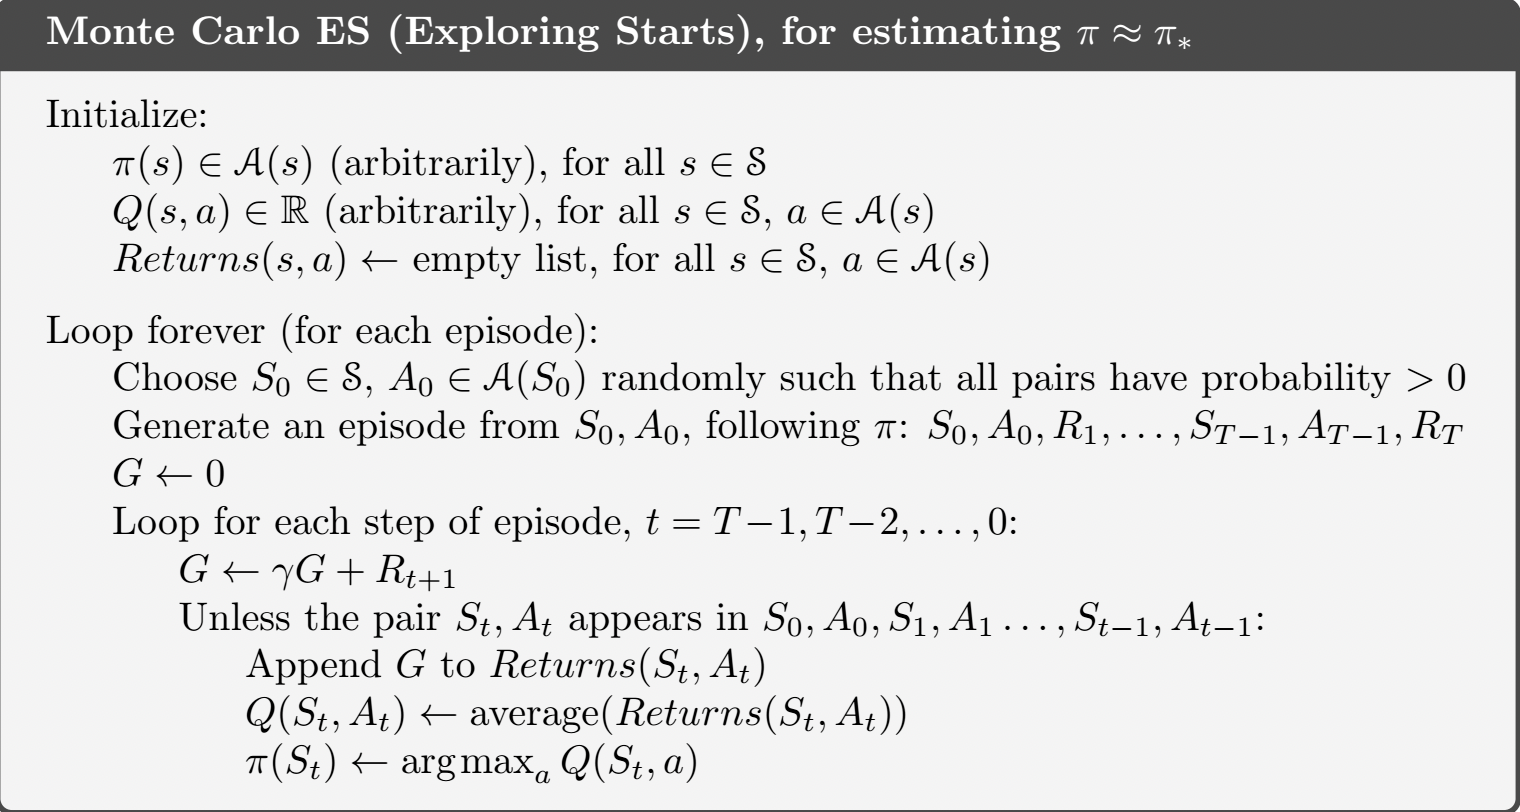
\includegraphics[width=350px,height=200px]{images/mc_es.png}
        \caption{Monte Carlo ES (Exploring Starts)}
        \label{fig:my_label}
    \end{figure}


\section{TD learning}

Temporal difference learning (TD) is an important concept in reinforcement learning and it combines a lot of the information that we have covered so far. It takes ideas from MC methods and dynamic programming. It can learn from experience like we saw in MC methods but also bootstraps like in DP. In the equations below we can see the differences between TD learning and MC Methods. The first equation is essentially what MC methods attempts to estimate. The last equation is what DP learning uses and also what TD learning uses. You can see how in the last equation we are bootstrapping by using a future estimate to approximate the current one. 

$$ \mathbf{v}_{\pi}(s) = \mathbb{E}_{\pi}[G_{t} | S_{t} = s] $$

$$ =  \mathbb{E}_{\pi}[R_{t + 1} + \gamma G_{t + 1} | S_{t} = s] $$

$$ =  \mathbb{E}_{\pi}[R_{t + 1} + \gamma \mathbf{v}_{\pi}(S_{t + 1}) | S_{t} = s] $$

In TD learning the last equation gives us our TD target and so in their most basic form TD methods make an update to a value function as follows. 

$$ V(S_{t}) \leftarrow V(S_{t}) + \alpha[R_{t + 1} + \gamma V(S_{t + 1}) - V(S_{t})] $$

We are using $V(S_{t})$ here to signify that we dont actually have access to $v_{\pi}$. Likewise the "target" for MC methods is generally $G_{t}$ and we sample the expected value in order to approximate it. In TD learning we are using sampling as well. We sample the expected value in the third equation and we also maintain an estimate of $v_{\pi}$. This is why we say that TD combines MC methods and DP. It uses the sampling of MC with the bootstrapping of DP. We can use this basic update above to give us a simple method for doing policy evaluation. 

\begin{figure}[H]
        \centering
        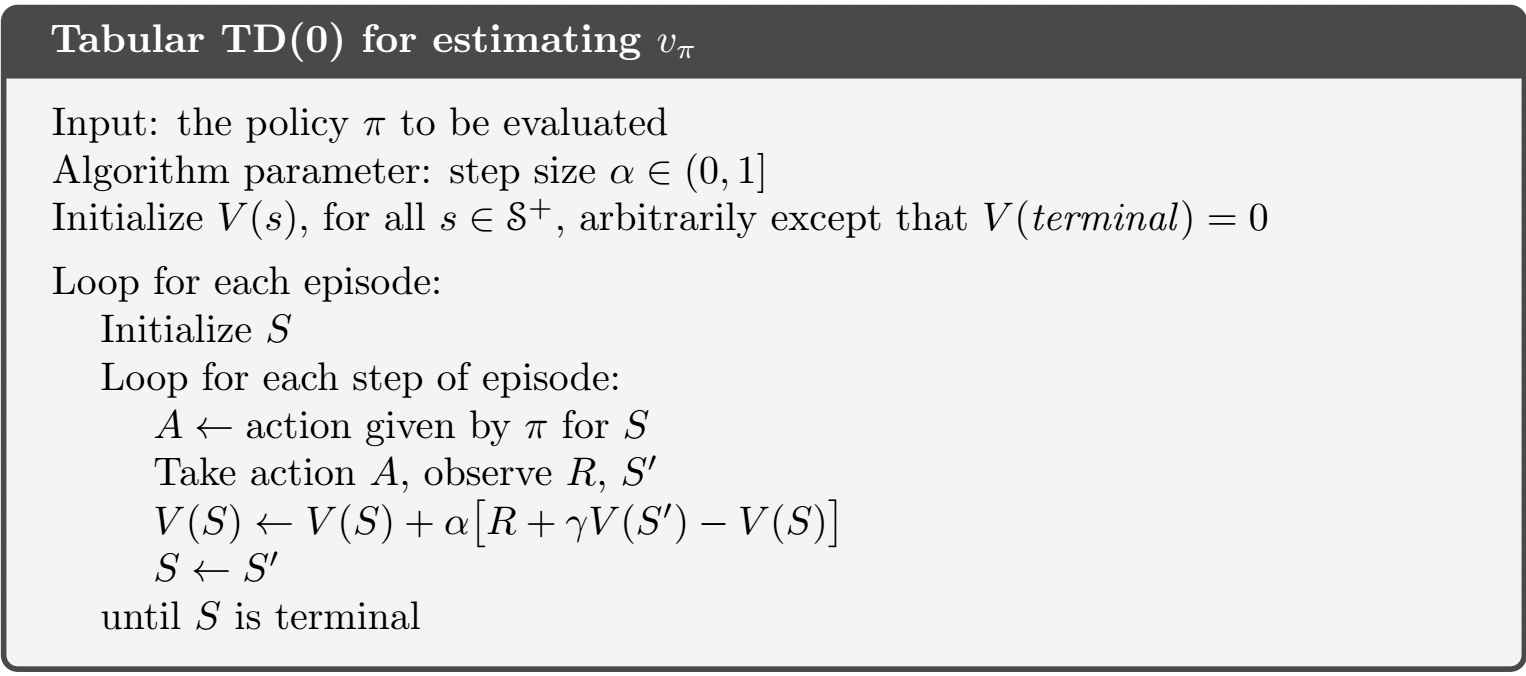
\includegraphics[width=350px,height=200px]{images/tabular_0.png}
        \caption{Tabular TD Sutton Chpt 6}
        \label{fig:my_label}
    \end{figure}
    

The difference here in the bootstrapping mechanism from that of DP is that a single sample of a successor state $V(S^{'})$ is used instead of looking at all possible next states. The quantity in brackets in the TD update is called the TD error and it comes up a lot in reinforcement learning. It is a sort of error because we have a target ($R_{t + 1} + \gamma V(S_{t + 1})$) and we have our estimate $V(S_{t})$. There is an interesting result here that if V(s) is not updated during an episode then we can actually write the Monte carlo error as a sum of TD errors

$G_{t} - V(t) = \sum_{k=t}^{T - 1} \gamma^{k - t}\delta_{k}$

Here $\delta_{k}$ is the TD error. $\delta_{k} = R_{k + 1} + \gamma V(S_{k + 1}) - V(S_{t})$

TD methods have some advantages over MC methods and DP methods. 

* TD > DP because no model of the environment is required. 
* TD > MC methods in that they are naturally implemented in an online, fully incremental fashion. Dont need to wait until the end of an episode. 
* Has similar convergence guarantees as DP and MC. 

Now just like with DP and MC methods we need to go from simply evaluating a policy to having a method for improving a policy. We will use the GPI as before as a framework for achieving this. Just like with MC we focused on estimating $q_{\pi} (s,a)$ which does not force us to have a model of the environment. The TD update can be rewritten in this notation as 

$ Q(S_{t}, A_{t}) \leftarrow Q(S_{t},A_{t}) + \alpha[R_{t + 1} + \gamma Q(S_{t + 1},A_{t + 1}) - Q(S_{t},A_{t})]$

This is an on-policy method since we are using our policy to sample actions $A_{t + 1}$ for our target value. The algorithm below is an example of an algorithm that utilizes this update. We can see that policy evaluation and policy improvement are coupled a bit more tightly than before. We are using the current value estimate Q(s,a) to find a greedy policy that serves as our policy improvement step. Then for policy evaluation we use the update previously described. 

\begin{figure}[H]
        \centering
        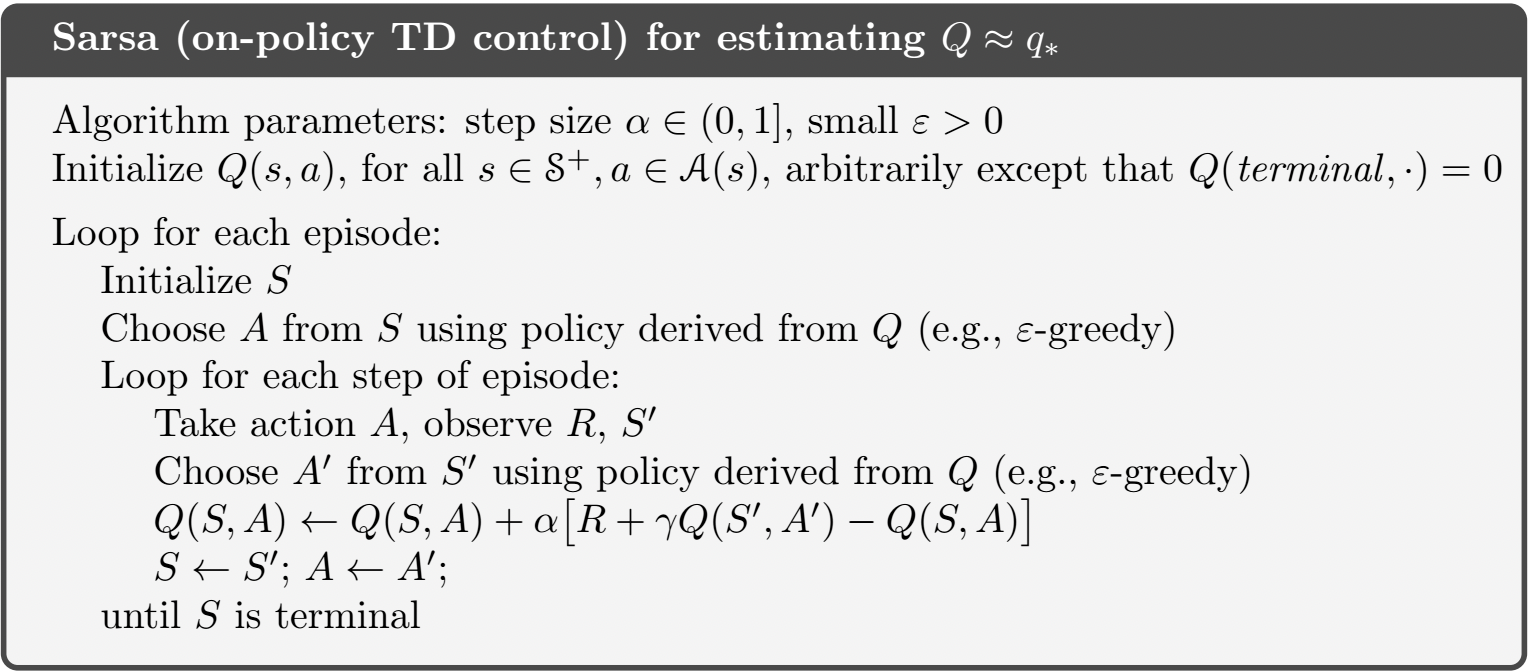
\includegraphics[width=350px,height=150px]{images/sarsa.png}
        \caption{Sarsa: Sutton Chpt 6}
        \label{fig:my_label}
    \end{figure}

A variant of Sarsa is called Q learning and has gained quite a bit of popularity since its recent success with its deep learning variant DQN which we will discuss later. Q learning modifies the TD target by simply taking the max action of the observed next state. So the TD error becomes. 

\begin{equation}
   \delta_{t} = R_{t + 1} + \gamma \: \underset{a}{max}Q(S_{t + 1},A_{t + 1}) - Q(S_{t},A_{s})
\end{equation}

The learned value function in this case directly approximates $q_{*}$. This is because it satisfies the policy improvement theorem by always taking the max action. It also still manages to visit all state action pairs by acting $\epsilon$-greedily from the current state. There have been a lot of nice theoretic work to prove convergence (Watkins,1989). The adjusted algorithm is presented in full below. The change to using the max action in place of an action selected from the policy means that we form a target that does not depend on the policy being used and therefore makes the algorithm an off-policy algorithm. So this off-policy distinction simply means that with off-policy we learn using a different policy than the one we used to take actions with. Q learning has had a lot of success when combine with deep learning which we will look at next. 

\begin{figure}[H]
        \centering
        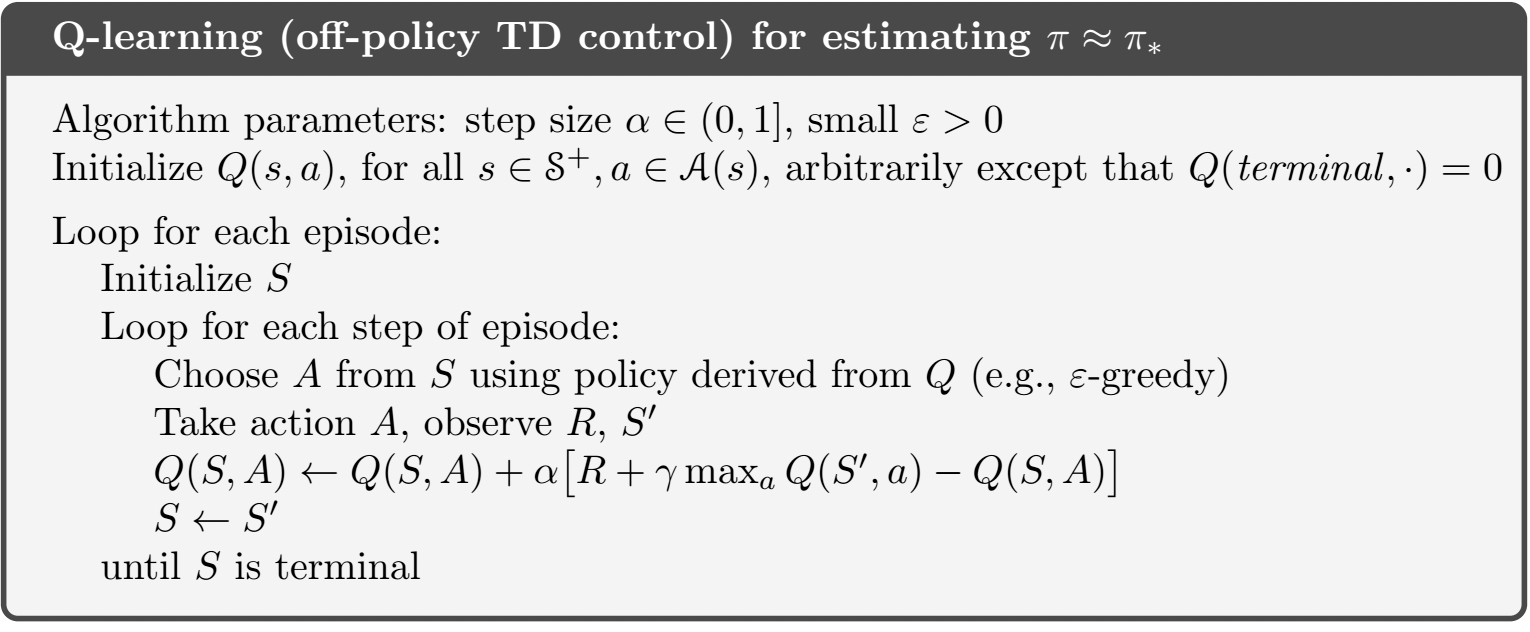
\includegraphics[width=350px,height=150px]{images/q_learning.png}
        \caption{Q learning: Sutton Chpt 6}
        \label{fig:my_label}
    \end{figure}
    
    
\section{Function approximation and Deep RL}

We have seen so far that no matter what the approach to RL is you need someway to evaluate a policy and you need a way to improve a policy. We also identified some of the bottlenecks of various approaches. DP for instance suffers from the "curse of dimensionality" in that as the size of the state space increases the computational requirement grows exponentially. Monte carlo methods and TD learning helped us to get around this by being able to effectively sample and learn from experience. We looked at tabular methods that essentially maintained a lookup table for each state action pair like in Q learning. This has its limits as the state and action space grows. It will become unfeasible to require approximating the value of Q(s,a) for every state and action pair. It requires too much computation to adequately approximate the true $q_{\pi}$ for a given policy. If the state space is large it is reasonable to think that an agent will often encounter states that it has never seen before even after a lot of exploration. What if we were able to generalize the information learned from one state to other similar states? This would allow us to more effectively make use of experience. This task of generalizing from a given set of data to unseen data has been studied quite a bit. Function approximation is the typical approach that helps us to learn from examples. 

Function approximation usually means that we attempt to parameterize a function with a set of learned weights. Parameterizing a function would mean that we take a set of weights $\mathbf{w} \in \mathbb{R}^{d} $ and use them to approximate the true value function $\mathbf{v}_{\pi}$ for a given policy $\pi$. This can be represented as $\hat{\mathbf{v}}(s,\mathbf{w}) \approx \mathbf{v_{\pi}}$. The function $\hat{\mathbf{v}}$ can be something complex like a neural network or something more simple like a linear function. Function approximation helps with generalization in that we now have a set of weights that "represent" the states. Instead of having a separate representation for each state we can represent many states with a lower dimensional representation since typically $d << |S|$. Two states that are similar by some metric will have a similar representation in this new weight space. That means that it should have a similar output as well. So if we have some similarity metric $d$ then if for two states $s_{1}$ and $s_{2}$ we have that $d(s_{1},s_{2}; \mathbf{w}) \approx 0$ then we also should have that $ | \hat{\mathbf{v}}(s_{1},\mathbf{w}) - \hat{\mathbf{v}}(s_{2},\mathbf{w}) | \approx 0$. Thinking to a tictactoe example you would want two board positions that are similar to have similar values. Such as the following two boards. 

\begin{figure}[H]
    \centering
    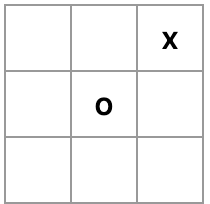
\includegraphics[width=100px,height=100px]{images/t_board_0.png}
    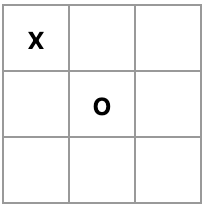
\includegraphics[width=100px,height=100px]{images/t_board_1.png}
    \caption{TicTacToe Board}
    \label{fig:my_label}
\end{figure}
    
Supervised learning is a common function approximation technique used in machine learning in which an algorithm is given a set of data $X$ and some labels $Y$ that are the thing the algorithm is attempting to learn. The goal is to find patterns in $X$ that allow one to be able to minimize some loss function $L(f(X^{'}),Y^{'})$ where the algorithm is represented by the function $f$ and $X^{'},Y^{'}$ is some unseen data but that come from the same distribution as the observed data $X$. Some of the difficulty in applying supervised learning techniques to reinforcement learning is that we actually are not looking at a stationary distribution. The parameters that describe the underlying distribution are capable of changing over time and as the agent interacts with the environment. To further highlight difficulties with using this approach in RL we are generally trying to do policy evaluation  using the current policy $\pi$. This however will be changing as we run policy improvement. So we must use methods that are able to handle the nonstationarity of the problem. 

Nevertheless we can start by phrasing our RL problem as a SL problem. First we need to actually specity our loss function for RL as well. We know that we want to minimize some distance between what our parameterized prediction says and what our target says. We want to specify $L (\mathbf{v}_{\pi},\hat{v}(s,\mathbf{w}))$. A common function for $L$ is the MSE. We can write this as $\mathbf{MSE} = \sum_{s \in S} [\mathbf{v}_{\pi}(s) - \hat{v}(s,\mathbf{w})]^{2}$. We dont have access to the underlying function $\mathbf{v_{\pi}}$ but we can use our target that we have specified in previous examples. In supervised learning terminology we have a target like $G_{t}$ (MC target) or $ R_{t + 1} + \gamma \hat{\mathbf{v}}(s,\mathbf{w})$ the TD target which is like our labels $Y$ and we have the current state $S_{t}$ which is like an observation of $X$

\section{DQN}

We have discussed briefly the idea of applying function approximation to RL. The task is non trivial and we have noted a couple of the dangers involved. I will now use a popular paper to further the discussion of the use of function approximation to enhance the ability of a RL algorithm to better generalize. A nature paper from 2015 entitled "Human-level control through deep reinforcement learning" showed how you could take a "simple" algorithm like Q learning and scale it to be a state of the art. Previous work on applying Neural networks to Q learning showed that this approach was unstable {RL is unstable paper}. The instability comes from several sources. 

\begin{itemize}
    \item Correlations present in the sequence of observations
    \item Small updated to Q may significantly change the policy and therefore the data distribution
    \item Correlations between action-values (Q) and the target values r + $\gamma Q(s^{'},a^{'})$
\end{itemize}

We have already mentioned the second issue which refers to the nonstationarity of the data. The other two refer to a common problem that most supervised learning (SL) problems are forced to address. That is correlation among samples. There is a common assumption made in most SL tasks that the observed samples are IID (Independentally and Identically distributed). A lot of care has to be taken to help at least approximate this assumption.  In the case of Q learning the sequences are highly correlated but so are the labels. The DQN paper address these issues in two ways. 

\begin{itemize}
    \item Using an experience replay buffer that randomizes the data
    \item Only periodically update Q and maintain a target network. 
\end{itemize}

The first helps to solve the first two problems. It helps remove correlation in the observations through random sampling of a replay buffer. We will discuss the details of the replay buffer shortly. The randomization also helps to solve the nonstationarity problem as it smooths out the data distribution. DQN only periodically updates the Q function which helps to remove correlation with the target values. Since a separate network is maintained for making target predictions this means that the target values remain much more stable. 

DQN uses a neural network to parameterize the state-action function $Q(s,a) \rightarrow Q(s,a,\theta_{i})$. Here $\theta_{i}$ signifies the parameters of the network at iteration $i$. Recall from our discussion of Q learning that the TD error had the form $\delta_{t} = R_{t + 1} + \gamma \: \underset{a}{max} Q(S_{t + 1},A_{t + 1}) - Q(S_{t},A_{t})$. In the DQN paper they translate this to a differentiable loss function as follows. 

$ \mathbf{L_{i}}(\theta_{i}) = \mathbb{E}_{s,a,r,s^{'} \sim \: U(D)} [(r + \gamma \: \underset{a}{max} Q(s^{'},a^{'};\theta_{i}^{-}) - Q(s,a;\theta_{i}))^{2}]$

The $\theta^{-}$ weights are the weights for the target network. This is simply the mean squared error of the target and predicted values using the parameterized version of the Q function. Note how the target value depends on the prediction of the target network. This is really a large distinction between reinforcement learning and supervised learning. A picture of their network used is given below. They evaluated their agent on Atari games and used a convolutional neural network for the parameterized Q function. The output of the network that you see on the far right is the set of possible actions with each of the corresponding values. 

\begin{figure}[H]
    \centering
    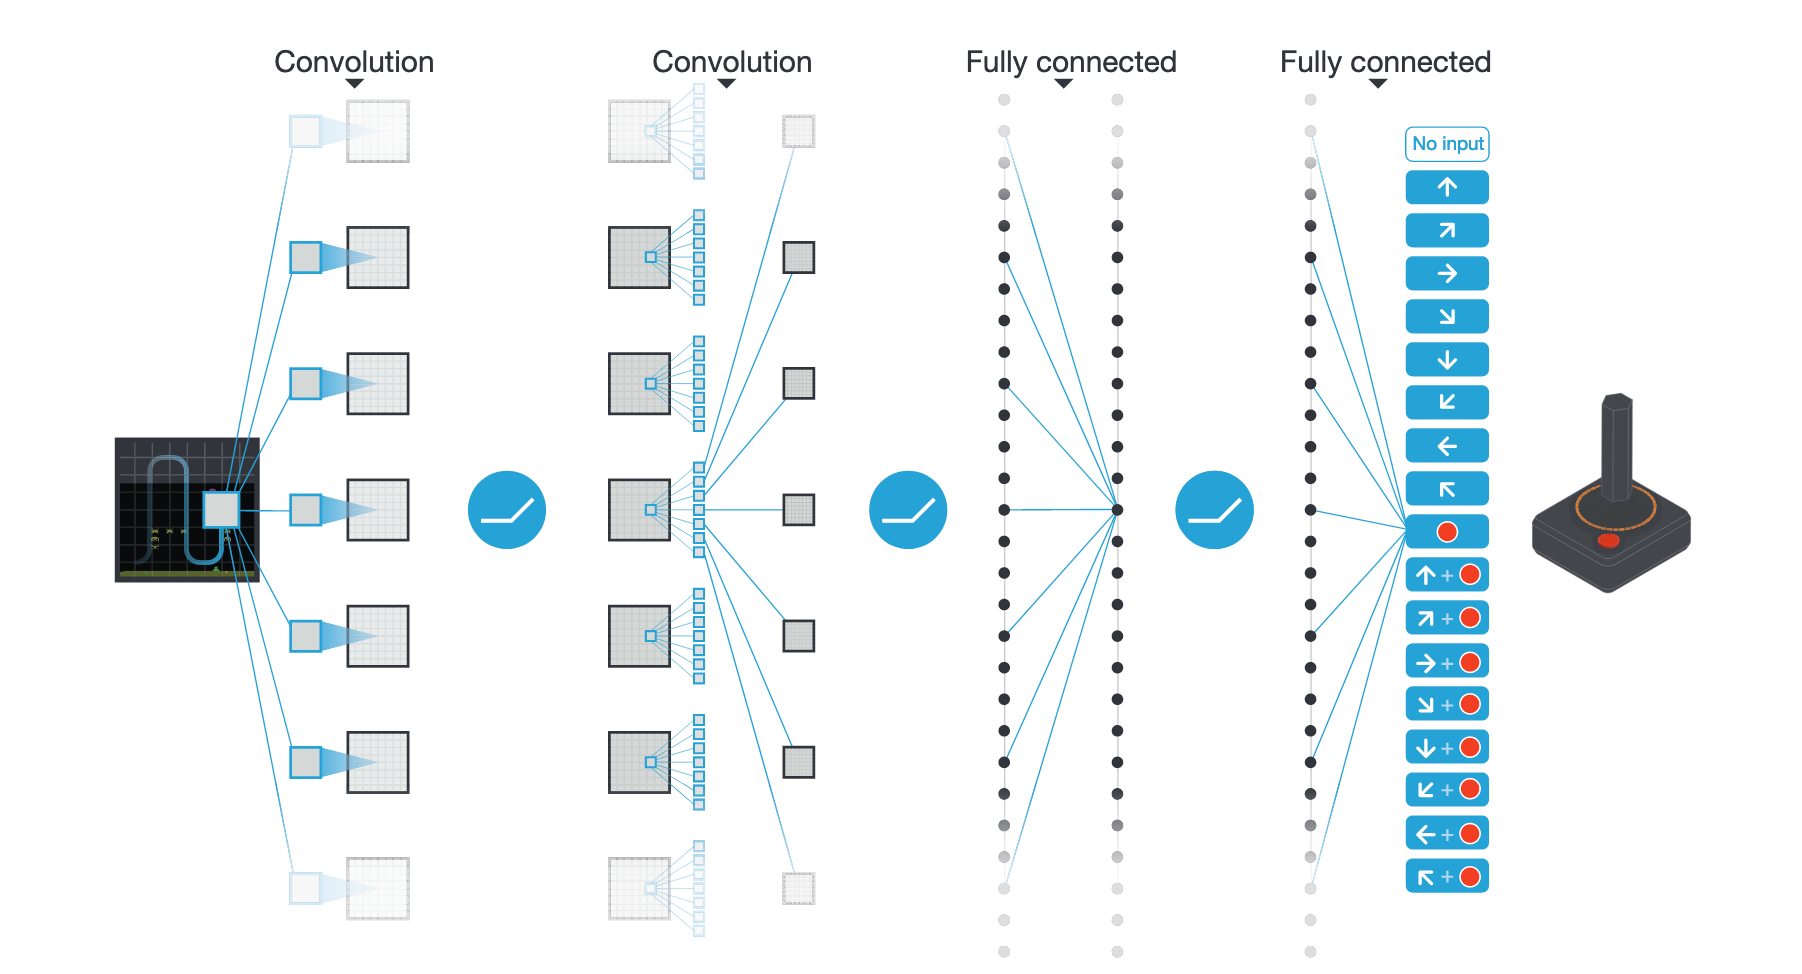
\includegraphics[width=350px,height=200px]{images/DQN_architecture.png}
    \caption{DQN architecture}
    \label{fig:my_label}
\end{figure}

Prior to looking at the algorithm in full lets look at two of the more important components that made DQN successful. First the target network being used requires a bit more explanation. To be clear its not actually a separate network. It is simply weights of the Q network at prior iterations. So it is basically "old" weights. We specify the number of iterations that we wait to update the target network up front as a hyper parameter. When we do finally update the target network we simply copy the current network weights and use them as our new target. This does not completely fix the nonstationary problem since in all RL algorithms that bootstrap we will always have some amount of variability in the target distribution. 

We also need to look at a what an experience replay buffer is. The experience replay buffer is essentially a database of experience. While the agent interacts with the environment data that is generated from that interaction is stored away. Then to update the network batches of experience are randomly sampled from the buffer. The fact that the experience is sampled randomly is significant in that it helps to decorrelate the data and stabilize training. Experience is typically stored in the form ($s_{t},a_{t},r_{t},s_{t + 1}$). The current state, action, reward and the next state that the agent transitions to after taking action $a_{t}$. A replay buffer will be used in the AlphaZero algorithm so keep it in mind going forward. 

The algorithm from the paper is in the figure below. Lets go through each one of the steps. It might look complicated but it is really quite similar to Q learning that we have seen plus some deep learning magic. 

\begin{figure}[H]
    \centering
    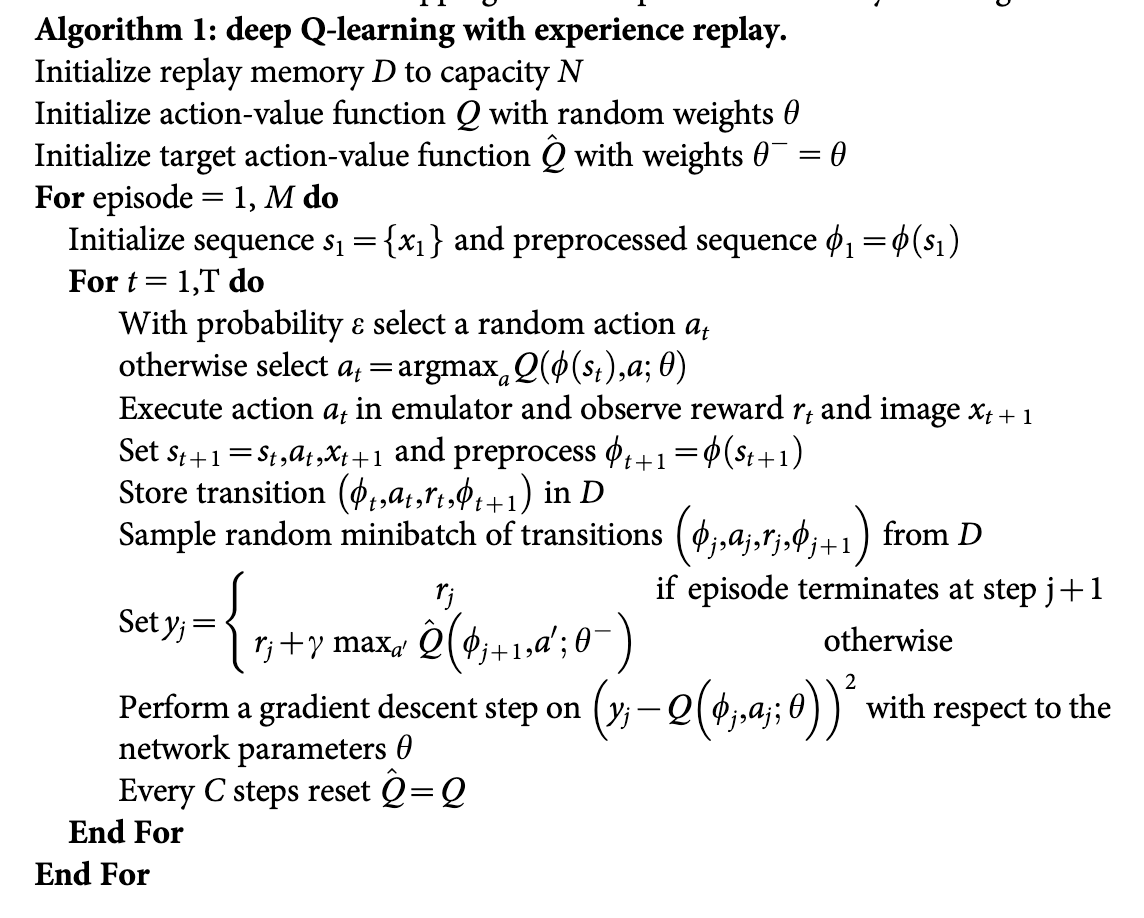
\includegraphics[width=350px,height=200px]{images/DQN_algo.png}
    \caption{The DQN algorithm}
    \label{fig:my_label}
\end{figure}

\begin{enumerate}
    \item Initialization - We simply initialize the weights of the network randomly and then set the target weights to a copy of those weights. We also initialize the replace buffer which simply means instantiating whatever data structure your using to hold the data such as an array.  
    \item Inside the main for loop we get the initial sequence. A sequence here is a stack of the 4 most recent frames. Then the function $\phi(s_{t})$ scales those frames to be of size 84 x 84. 
    \item The second for loop takes us through each step of the episode. We use an $\epsilon$-greedy strategy to select an action. The action is executed against the environment and the reward and next state are observed and processed. 
    \item We store the current data into the replay buffer. 
    \item We train our network on a random sample of transitions from our replay buffer using gradient decent and the previously discussed loss function. 
\end{enumerate}

Thats really it. This is something that you can code up in less than 150 lines of python code using a modern machine learning framework like pytorch or tensorflow. This seemed like a nice elegant algorithm that utilized deep learning to reach state of the art performance on difficult tasks like the Atari games. So why not use this same approach to solve something like Go? There is something that this approach still suffers from. It has difficulty with the credit assignment problem and stability in sparse reward regimes. The credit assignment problem in RL is the problem of knowing whcih action in which state was responsible for a particular outcome. In a game like Go you will generally take many many actions prior to the end of the game and wont receive any feedback until the game is complete. This is what is meant by sparse rewards. The lack of informative feedback from the environment. Once the game is complete you will know wheter you won or lost (+1,-1). Then how do you inform the network which states and actions were responsible for the outcome? In theory its not totally obvious why the Deep Q learning algorithm should not be able to overcome these issues. In absence of better theory however we must be content with the empirical evidence that points to DQN's instability in these regimes. We now will discuss the idea of planning and how that helps to overcome this problem. AlphaZero is a complex planning algorithm so we will start with something a bit more simple. 